\documentclass[a4paper,11pt]{report}
\usepackage[T1]{fontenc}
\usepackage[utf8]{inputenc} 
\usepackage[english]{babel} 
\usepackage{url}
\usepackage{graphicx}
\usepackage{lipsum}
\usepackage{tocbibind} 
\usepackage{booktabs}
\usepackage{colortbl}
\usepackage[table]{xcolor}
\setlength{\arrayrulewidth}{0.5mm}
\setlength{\tabcolsep}{18pt}
\renewcommand{\arraystretch}{2.5}
\usepackage{longtable}
\usepackage{array}
\newcolumntype{C}[1]{>{\centering\let\newline\\\arraybackslash\hspace{0pt}}m{#1}}
\usepackage{url}							
\usepackage{hyperref}
\usepackage{enumitem}
\usepackage{float}
\restylefloat{table}
\usepackage{xltabular}
\usepackage{xcolor}
\definecolor{green1}{HTML}{85AB67}
\definecolor{green2}{HTML}{77BC3F}




\begin{document}

\begin{titlepage}

\newcommand{\HRule}{\rule{\linewidth}{0.1mm}}

\center 


\includegraphics[width=50mm,scale=0.5]{./Images/Logo_Politecnico_Milano.png}\\[0.5cm] 

{\Large Computer Science and Engineering}\\[0.4cm] 
{\large Software Engineering 2}\\[0.4cm] 
{\large Academic year 2021-2022}\\[0.5cm] 

\HRule \\[1.5 cm]
{\LARGE Requirements Analysis and Specification Document} \\[1cm]
{\textbf {\Huge DREAM}}\\[0.3cm] 
{\LARGE Data-dRiven PrEdictive FArMing in Telangana} \\[1cm]
\HRule \\[1.5cm]
\raggedright

\begin{minipage}{0.55\textwidth}
\begin{flushleft} \large
\emph{Authors:}\\
Arslan \textsc{Ali}\hfill 971503 \\
Elisa \textsc{Servidio}\hfill 996387 \\
Federica \textsc{Suriano}\hfill 953085 \\
\end{flushleft}
\end{minipage}\\[1 cm]
~

\center

{\large - -, 2021}\\[0.3 cm]
{\large Version -.0}\\

\vfill 
\end{titlepage}

\newpage

\addtocontents{toc}{\protect\setcounter{tocdepth}{-1}}
\tableofcontents
\addtocontents{toc}{\protect\setcounter{tocdepth}{3}}
\listoftables
\newpage
\listoffigures
\newpage

\chapter{Introduction}

The Requirement Analysis and Specification Document (RASD) has the purpose of describing, to a wide range of potential readers, the system to be developed for the problem under consideration.\\ 
It contains the description of the scenarios, the corresponding use cases and the models describing requirements and specifications.\\
It focuses also on interactions between the system and the users, including the implied  constraints and functionalities that are going to be implemented.

\section{Purpose}

Telangana is the 11th largest and the twelfth-most populated state in India with a geographical area of 112,077 km2 and 35,193,978 residents (data from2011).
The economy of Telangana is mainly driven by agriculture, a sector which plays a pivotal role in all India’s economy: over 58\% of rural households depend on it as the principal means of livelihood, 80\% of whom are smallholder farmers with less than 2 hectares of farmland. More than a fifth of the small-holder farm households are below poverty. \\

Worldwide there are many threats to the agriculture sector.\\ World population is estimated to reach 9.7 billion by 2050, therefore food demand is expected to increase anywhere between 59\% to 98\% by 2050.Climate change is predicted to result in a 4\%-26\% loss in net farm income towards the end of the century. The COVID-19 pandemic has greatly exposed the vulnerabilities of marginalized communities, small holder farmers and the importance of building resilient food systems.\\

This calls for a revamp of the entire food supply chain to help bolster countries against shocks and challenges. For this reason, Telangana’s government aims to design, develop and demonstrate anticipatory governance models for food systems using digital public goods and community-centric approaches to strengthen data-driven policy making in the state. To achieve this goal, Telangana wants to partner with IT providers with the aim of acquiring and combining data concerning: weather forecasts, agriculture production (types and produced amount per product, amount of water used by each farmer), humidity of soil and information provided by the governmental agronomists. Acquiring and combining such data, the software system DREAM supports the work of three types of actors: policy makers, farmers, and agronomists.\\

DREAM allows Telangana’s policy makers to identify farmers who are performing well and those who are performing particularly badly. The first ones, especially the more resilient to meteorological adverse events, will receive special incentives and will be asked to provide useful best practices to the others. Moreover, the system will help policy makers to understand whether the steering initiatives carried out by agronomists with the help of good farmers produce significant results.
Thanks to the application the policy makers will be able to make decisions in the real world by analyzing and visualising data regarding farmers.\\

On the other hand, farmers are allowed to visualize data relevant to them based on their location and type of production, such as weather forecasts and personalized suggestions (i.e. specific crops to plant or specific fertilizers to use). Farmers can insert in the system data regarding their production and any problem they face. They can also request for help and suggestion by agronomists and other farmers with whom they can also create discussion forums.\\

Eventually, agronomists are in charge of a certain mandal, which is a local government area and administrative division of Telangana. They can receive information about requests for help and answer them and they can visualize data concerning weather forecasts and farmers in the area. Furthermore, agronomists can visualize, up-date and confirm a daily plan to visit farms, assuming that all farms must be visited at least twice a year, but those that are under-performing should be visited more often, depending on the type of problem they are facing.

\subsection{Goals of the Application}
\begin{itemize}
    \item [\textit {G.1}] Allows policy makers to visualize and analyze data of farmers
    \item [\textit {G.2}] Allows policy makers to identify those farmers who are performing well
    \item [\textit {G.3}] Allows policy makers to identify those farmers who are performing badly
    \item [\textit {G.4}] Allows policy makers to verify the improvement of farmers who have been already helped by agronomist or good farmers
    \item [\textit {G.5}] Allows farmers to visualize data and suggestions relevant to them based on their location and type of production
    \item [\textit {G.6}] Allows farmers to insert in the system data about their production and any problem they face
    \item [\textit {G.7}] Allows farmers to request for help and suggestions by agronomists and other farmers
    \item [\textit {G.8}] Allows farmers to create discussion forums with the other farmers
    \item [\textit {G.9}] {\color{orange}  Allows agronomists to receive information about requests for help}
    \item [\textit {G.10}] Allows agronomists to answer to requests for help from farmers
    \item [\textit {G.11}] Allows agronomists to visualize data concerning farmers in the mandal
    \item [\textit {G.12}] Allows agronomists to visualize weather forecasts in the mandal
    \item [\textit {G.13}] Allows agronomists to visualize a daily plan to visit farms in the mandal
    \item [\textit {G.14}] Allows agronomists to update a daily plan to visit farms in the mandal
    \item [\textit {G.15}] Allows agronomists to confirm the execution of the daily plan at the end of each day 
    \item [\textit {G.16}] Allows agronomists to specify the deviations from the daily plan at the end of the day

\end{itemize}
\section{Scope}

The aim of the DREAM software product is to develop and adopt anticipatory governance models for food systems to strengthen data-driven state policy. \\
It takes care of the acquisition and management of all data collected in order to support the work of farmers, agronomists and policy makers.\\
The system aims to collect data not only from sensors located throughout the territory, but also from farmers. The analysis of the acquired data aims to improve the production of farmers.\\ Low-performing farmers are identified by policy makers and helped by the best-performing ones.\\
Everything is supervised by agronomists who take care of their own geographical areas of competence.\\

To better understand all the phenomena involved, we distinguish them into two types according to the World and Machine paradigm [M. Jackson and P. Zane]. The World is the environment surrounding the system, while the Machine is the system itself.

\subsection{World and Shared phenomena}

\begin{center}
    
\setlength\tabcolsep{7pt}
\rowcolors{2}{white}{white!65!green2!50}
\renewcommand{\arraystretch}{2}
\begin{longtable}{ |m{7cm}|C{2.3cm}|C{1.6cm}|}
\caption{World and Shared phenomena\label{long}}\\
\hline
\endfirsthead
\endhead
\hline
\endlastfoot
\rowcolor{green2}
\textbf{Phenomenon} & \textbf{Who controls it?} & \textbf{Is it shared?}\\
\hline

A farmer signs up to the application or logs in if already registered & W & Y\\
Telangana government assigns to each agronomist his ID code & W & N\\
An agronomist registers into the application by using his ID code or logs in if already registered & W & Y\\
Telangana government assigns to each policy maker his ID code & W & N\\
\textcolor{green}{The system checks validity of ID code} & M & Y\\
A policy maker registers into the application by using his ID code or logs in if already registered & W & Y\\
The system processes the performance of a farmer (or more than one) & M & N\\
A policy maker visualizes the performance trend of a farmer (or more than one) over time & W & Y\\
A policy maker visualizes the performance score of a farmer (or more than one) & W & Y\\
\noalign{\global\arrayrulewidth=0.3mm}
\arrayrulecolor{gray}\hline
The system notifies a farmer who is not performing well that it would be a good idea to request for help to an agronomist or a well performing farmer & M & Y\\
The system notifies a farmer that he improved his performance and he is entitled to receive an incentive & M & Y\\
The system retrieves longitude and latitude from the address of a farmer's land & M & N\\
The system sends personalized suggestions to a farmer based on computed data & M & Y\\
\textcolor{green}{The system retrieves weather forecasts, humidity of soil and amount of water used corresponding to a certain position} & M & Y\\
A farmer visualizes relevant information which are: weather forecasts, soil moisture and personalized suggestions and visits & W & Y\\
A farmer insert in the system the production of a certain period and the corresponding relevant data &  W & Y\\
\textcolor{green}{A farmer makes a help request} & W & Y\\
\textcolor{green}{The system assigns the help request to an agronomist and/or a well performing farmer} & M & N\\
A farmer opens a thread about a topic on the dedicated forum & W & Y\\
A farmer calls the agronomist to reschedule a visit & W & N\\
The system associates each farmer to the corresponding mandal & M & N\\
\noalign{\global\arrayrulewidth=0.3mm}
\arrayrulecolor{gray}\hline
An agronomist inserts in the system the mandal he is responsible of & W & Y\\
An agronomist receives a help request from a farmer & M & N\\
An agronomist replies to the help requests sent to him by farmers & W & Y\\
An agronomist calls a farmer to cancel a visit & W & N\\
An agronomist visualizes data about farmers of his mandal & W & Y\\
An agronomist visits a farm belonging to his mandal & W & N\\
An agronomist visualizes weather forecasts on the app & W & Y\\
The system creates the agronomist's daily plan, guaranteeing at least two visits per year for each farmer & M & N\\
An agronomist visualizes his daily plan & W & Y\\
An agronomist updates his daily plan & W & Y\\
An agronomist carries out his daily plan & W & N\\
An agronomist confirms his daily plan execution & W & Y\\
An agronomist specifies deviations from his daily plan at the end of the day & W & Y\\

\end{longtable}

\end{center}
\section{Definitions, Acronyms, Abbreviations}

In the following section is clarified the meaning of some definitions, acronyms and abbreviations which will be use in the RASD, in order to help the general understanding of the document.

\subsection{Definitions}
\begin{center}
\setlength\tabcolsep{7pt}
\rowcolors{2}{white}{white!65!green2!50}
\renewcommand{\arraystretch}{2}
\begin{longtable}{|m{3.2cm}|m{8.3cm}|}
\caption{Definitions}\\
\hline
\endfirsthead
\endhead
\hline
\endlastfoot
\hline
\textit{The System} & The whole system to be developed \\
\textit{User} & A farmer/agronomist/policy maker who uses the application\\
\textit{Application Service} & Functionality offered by the 
System for certain users \\
\textit{Policy Maker} & The user of the application who decides about new policies for Telangana \\
\textit{Farmer} & The user of the application who owns or manages a farm\\
\textit{Performance} & Indicator of the progress of a farmer's activity up to a certain date. Its value is calculated as numerical score \\
\textit{Score} & Is the performance rating computed by a function that depends on: type and quantity of harvested product, weather conditions, quantity of water consumed, soil moisture.\\
\textit{Well Performing Farmer} & A farmer who has a score higher than a certain threshold\\
\textit{Bad Performing Farmer} & A farmer who has a score below a certain threshold\\
\textit{Best Performing Farmer} & A farmer who has performed better than all the other farmers taken into consideration\\
\noalign{\global\arrayrulewidth=0.3mm}
\arrayrulecolor{gray}\hline
\textit{Agronomist} & The user of the application dealing with the management of a certain mandal\\
\textit{Mandal} & A local government area and  administrative division. Telangana is subdivided into districts which are themselves subdivided into mandals\\
\textit{Daily Plan} & Application service that allows the agronomist to manage his daily work schedule. Specifically, it allows him to track and organize visits to farmers\\
\textit{Discussion Forum} & Application service which a farmer can use to exchange ideas and opinions about a topic \\
\textcolor{red}{\textit{Thread}} & \\
\textcolor{red}{\textit{Post}} & \\
\textit{Help Request} & Application service which a farmer can use to request for help and suggestions to the agronomist or/and other well performing farmers\\
\hline
\end{longtable}
\end{center}
\subsection{Acronyms}

\begin{center}
\setlength\tabcolsep{7pt}
\rowcolors{2}{white}{white!65!green2!50}
\renewcommand{\arraystretch}{2}
\begin{longtable}{|m{1.5cm}|m{8.6cm}|}
\caption{Acronyms}\\
\hline
\endfirsthead
\endhead
\hline
\endlastfoot
\hline
\textit{DREAM} & Data-dRiven PrEdictive FArMing in Telangana\\
\textit{RASD} & Requirement Analysis and Specification Document\\ 
\textit{UML} & Unified Modelling Language\\
\textit{API} & Application Programming Interface\\
\hline
\end{longtable}
\end{center}
\subsection{Abbreviations}

\begin{center}
\setlength\tabcolsep{7pt}
\rowcolors{2}{white}{white!65!green2!50}
\renewcommand{\arraystretch}{2}
\begin{longtable}{|m{1.5cm}|m{8.6cm}|}
\caption{Abbreviations}\\
\hline
\endfirsthead
\endhead
\hline
\endlastfoot
\hline
\textit{G.i} & i-th goal\\
\textit{R.i} & i-th requirement\\
\textit{D.i} & i-th domain assumption\\
\textit{UC.i} & i-th use case\\
\hline
\end{longtable}
\end{center}
\section{Revision History}
\begin{center}
\setlength\tabcolsep{7pt}
\rowcolors{2}{white}{white}
\renewcommand{\arraystretch}{1.5}
\begin{longtable}{|p{1.5cm}|p{1.6cm}|p{2.75cm}|p{2cm}|}
\caption{Revision History}\\
\hline
\endfirsthead
\endhead
\hline
\endlastfoot
\rowcolor{green2}
\textbf{Version} & \textbf{Date} & \textbf{Authors} & \textbf{Summary}\\
\hline
1.0 & --/--/2021 & Arslan Ali &  First release\\
& & Elisa Servidio & \\
& & Federica Suriano &\\
\hline
\end{longtable}
\end{center}
\section{Reference Documents}

\begin{itemize}
    \item Specification document: “R\&DD Assignment A.Y. 2021/2022”
    \item Software Engineering 2 course slides
    \item EEE Std 830-1998: IEEE Recommended Practice for Software Requirements Specifications
\end{itemize}



\section{Document Structure}

The RASD is structured in the following five chapters:
\begin{itemize}
\item \textbf{Chapter 1 -  \textit{Introduction}:} It contains a general introduction to the problem of interest and a more detailed list of the goals of this project. The scope of the application is described thanks to the analysis of the phenomena involved.
A part relating to the definitions used in the document is also included.

\item \textbf{Chapter 2 -  \textit{Overall Description}:} It contains an overall description of the project including some possible scenarios of interest, the system class diagram and state diagrams.
The most important product functions necessary for the correct functioning of the application and all the assumptions on the domain are also described.

\item \textbf{Chapter 3 -  \textit{Specific Requirements}:} In this part the software product requirements are described in detail.
The description of the interfaces is included and the functional requirements are defined thanks to the use of UML diagrams.
This section also includes performance requirements, design constraints and software system attributes.

\item \textbf{Chapter 4 -  \textit{Formal Analysis using Alloy}:} It contains formal modeling of the software product using the Alloy tool and dedicated comments to better clarify each part of the modeling.

\item \textbf{Chapter 5 -  \textit{Effort Spent}:} It contains all the information regarding the hours of work required to create the document and the tasks assigned to each person in the team.
\end{itemize}

At the end of the document the bibliography is also included.

\chapter{Overall Description}

This chapter contains a general description of the system from a high level point of view. \\
It describes the general factors that affect the product and its requirements. It does not state specific requirements. Instead, it provides them a background, which is useful to define them in detail in \textit{Chapter 3}.\\
Starting from scenarios and domain models, it proceeds with an analysis of product functions and users' most relevant needs in order to define assumptions, dependencies and constraints of the entire application system.



\section{Product Perspective}
In subsection \textit{2.1.1} are listed the most relevant scenarios which are a narrative description of what users do and experience as they try to make use of the application.\\
They provide a general depiction of how major components of the system and users interact.\\
Moreover, in subsections \textit{2.1.2} and \textit{2.1.3} the domain of the system is defined through different models using UML.

\subsection{Scenarios}

\begin{enumerate}

\item Scenario: \textbf{Sunil discovers DREAM}\\\\
Sunil is a farmer from Telangana. Unfortunately, due to the adverse and unpredictable effects of climate change, his production of black carrots is gradually decreasing. Sunil learns from a colleague of his that there is an application called DREAM that could help him. Sunil registers and logs in, hoping to profit from it and improve his production.\\

\item Scenario: \textbf{Rajesh looking for advice}\\\\
Rajesh is a landowner from Adilabad district in Telangana, he owns several agricultural properties in the city. After his recent business trip to Russia, where he attended the beet fair, he is convinced to plant beets on his land too. As this is a little-known plant in the area, he doesn't know who to ask for advice. Rajesh's son Ram, also in the agricultural sector for several years, advises his father to use DREAM since Rajesh already had an account registered with the application.
Rajesh consults on the application the discussions already opened by other Telangana farmers to see if any of them had ever sought advice on beet cultivation. Unfortunately he cannot find any, so thanks to the suggestion of his son Ram he decides to open a thread on the dedicated forum, so that he can ask for advice about the plant from other farmers throughout Telangana.\\

\item Scenario: \textbf{Anita and her strategic plan}\\\\
Anita is the administrator of her mandal Sarangapur, in Jagtial district, as an inspector of production and development of the primary sector. Sarangapur is characterized by great periods of drought, so water is a particularly precious resource for citizens.
Recent analyzes have shown that over 90\% of the water is used by farmers.
Anita discovers DREAM and she wants to monitor the water consumption within each mandal in Telangana over the current year. Her goal is to identify the one that consumes the least water to study its strategies, so she enters the parameters of interest (quantity of water and Telangana mandals) on the application.
At this point the app returns the mandals and the corresponding consumed water in this last year and Anita is pleased to discover that the primacy is Pegadapalli, a mandal from her own district.\\

\item Scenario: \textbf{Manoj, the Indian tycoon}\\\\
Manoj is an Indian tycoon who would like to invest his capital in the agricultural sector. He accesses the DREAM application as policy maker and checks the map showing the performance score of each mandal. Manoj identifies the best performing ones and decides to invest in Geesugonda mandal which is located in Warangal district.\\

\item Scenario: \textbf{Mahima is thrilled with joy for DREAM}\\\\
Mahima is the Additional Director of Agriculture who assist the state Head quarter Commissioner\&Director of Agriculture in Telangana. She belongs to the Department of Agriculture, which provides agricultural services to farmers and aims to transfer the latest technical knowledge to the farming community. She was one of those who pushed for the creation of DREAM.
Mahima is thrilled with joy for its market launch and she is looking forward to use the application, therefore she gets her personal ID code to be able to registers with the role of policy maker and logs into DREAM.\\

\item Scenario: \textbf{A new job for Shanti}\\\\
Shanti is a young agronomist who operated in Palakeedu, a mandal in Suryapet district. She sees the announcement published on the Telangana government website in which it is reported that the DREAM application has been launched on the market and that for each mandal is required an agronomist. She is unemployed and interested in filling this role. Therefore, she sends her CV, gets hired and receives her personal ID code which allows her to register into DREAM. Eventually, she inserts Palakeedu as mandal of her competence.\\

\item Scenario: \textbf{Champak tries natural farming}\\\\
Champak is a farmer who has planted wheat. The last crop was poor because he didn't have enough money to buy suitable pesticides. He still can't afford them, however he cannot suspend his agricultural activity since his family depends on it as the principal means of livelihood. For this reason Champak creates a help request to both the agronomist and well performing farmers. The first to answer is Jayapal, a well performing farmer from his same mandal. Jayapal suggests him to plant potatoes instead of wheat because they are more resistant. However, Champak has already planted wheat therefore changing crops is out of the question. Champak waits for other answers until Rajat, the agronomist, replies suggesting him to cover the seeds with microorganisms obtained from particular formulations of cow dung. Champak is willing to follow the advice and is satisfied with the answer. He marks the help request as solved. 
\\

\item Scenario: \textbf{The busy life of Aruna}\\\\
Aruna is the DREAM agronomist responsible for Jaipur mandal in Mancherial district. It is early morning and the working day is about to begin. Aruna consults the daily plan to check which are the scheduled visits for the day. An appointment with the farmer Gangesh is scheduled for the afternoon. At that moment she receives a phone call from him, who informs her that his wife is not well, he has to take her to the doctor and for this he has to cancel the scheduled visit. Aruna wishes him the best and updates the daily plan, cancelling the appointment. Further on, she completes all the appointments scheduled in the morning and she drives her car to reach Jaya, a farmer. Unfortounately, Aruna has a small accident with her car, she is unharmed but she will miss the appointment. She informs Jaya and calls a mechanic. She finally returns home in the evening and confirms the daily plan, also specifying the deviation corresponding to the missed visit due to the accident. She also has to reschedule in the first two free slots in her agenda the appointments with Jaya and Gangesh. To do so, she updates the daily plan of the next day. 
\\
\item Scenario: \textbf{Durvish, the inspector}\\\\
Durvish is the administrative head of Doma mandal, in Vikarabad district. The DREAM application was launched on the market the year before and now he wants to understand whether the steering initiatives carried out by agronomists with the help of good farmers have produced significant results. Therefore, Durvish accesses DREAM with his account and he enters the parameters of interest on the application to select only farmers of his mandal with at least an Help Request solved.
At this point the app returns the selected farmers. Durvish wants to visualize their general trend of the performance score as indicator of the efficiency of the application. He selects score as attribute and mean as operation, in return a time chart is shown. He pleasantly discovers that, except for an initial fluctuating trend, the general performance score of farmers with at least a solved Help Request of his mandal is constantly growing, a sign of effective usefulness of DREAM.
\\

\item Scenario: \textbf{Deepa fights soil salinity}\\\\
Deepa is a farmer of Telangana who is already using the application DREAM. The cotton she planted is now ready for harvest. The amount of cotton obtained from her hectare of land results in 3 bales, which correspond approximately to 107 kg each. Deepa accesses the app, selects the date corresponding to the current day and inserts in the system type and quantity of product harvested. Two days later, while approaching to plant cotton seeds again, she has a problem regarding the salinity of the soil which is particularly high and would not allow cotton to grow. For this reason, Deepa stores this information in the system selecting the current day, also adding that it was necessary to buy a biostimulant whose formulation neutralizes excess salts within the soil.
\\

\item Scenario: \textbf{Haresh's first encounter with coffee}\\\\
Haresh is a farmer of Telangana who is already using the application DREAM. It is October and within a few days he will have to harvest the sorghum he has planted. To better organize the work of the next few days, Haresh accesses the application and checks the weather forecasts. After the harvest he will also have to decide what to plant, which is why he also checks the soil moisture. Furthermore, due to the drought expected for November, the app suggests Haresh to plant coffee, a product that does not require a particularly humid soil. Haresh thinks that it could be a good idea, however he has never cultivated coffee so it could be necessary to confront with the agronomist about some technical details. Haresh doesn't remember when his next visit with the agronomist will occur, therefore he accesses the visits page on the application and pleasantly reads that one is scheduled for November 5th.
\\

\item Scenario: \textbf{Lohit helps the most needy}\\\\
Lohit is the DREAM agronomist responsible for Raipole mandal in Siddipet district. The performance score in his mandal for a good percentage of farmers has been around a value that has not been particularly high for more than six months. For this reason Lohit wants to visualize data regarding best performing farmers to formulate strategies to be applied to the most needy. He accesses DREAM and visualizes farmers whose performance score is between the highest. Analyzing the corresponding data he finds out that they cultivate all the same type of product: rice, which is cultivable under widely varying conditions but prefers hot and humid climate. Therefore, before advising other farmers to plant rice, Lohit consults weather forecasts and humidity of soil trend, discovering that with a very high probability there will be the perfect conditions in the next weeks.
\\

\end{enumerate}

\newpage
\subsection{Class Diagram}
In this section is reported the Class Diagram of the System, whose main concepts are presented from a high-level point of view. 
\begin{figure}[H]
  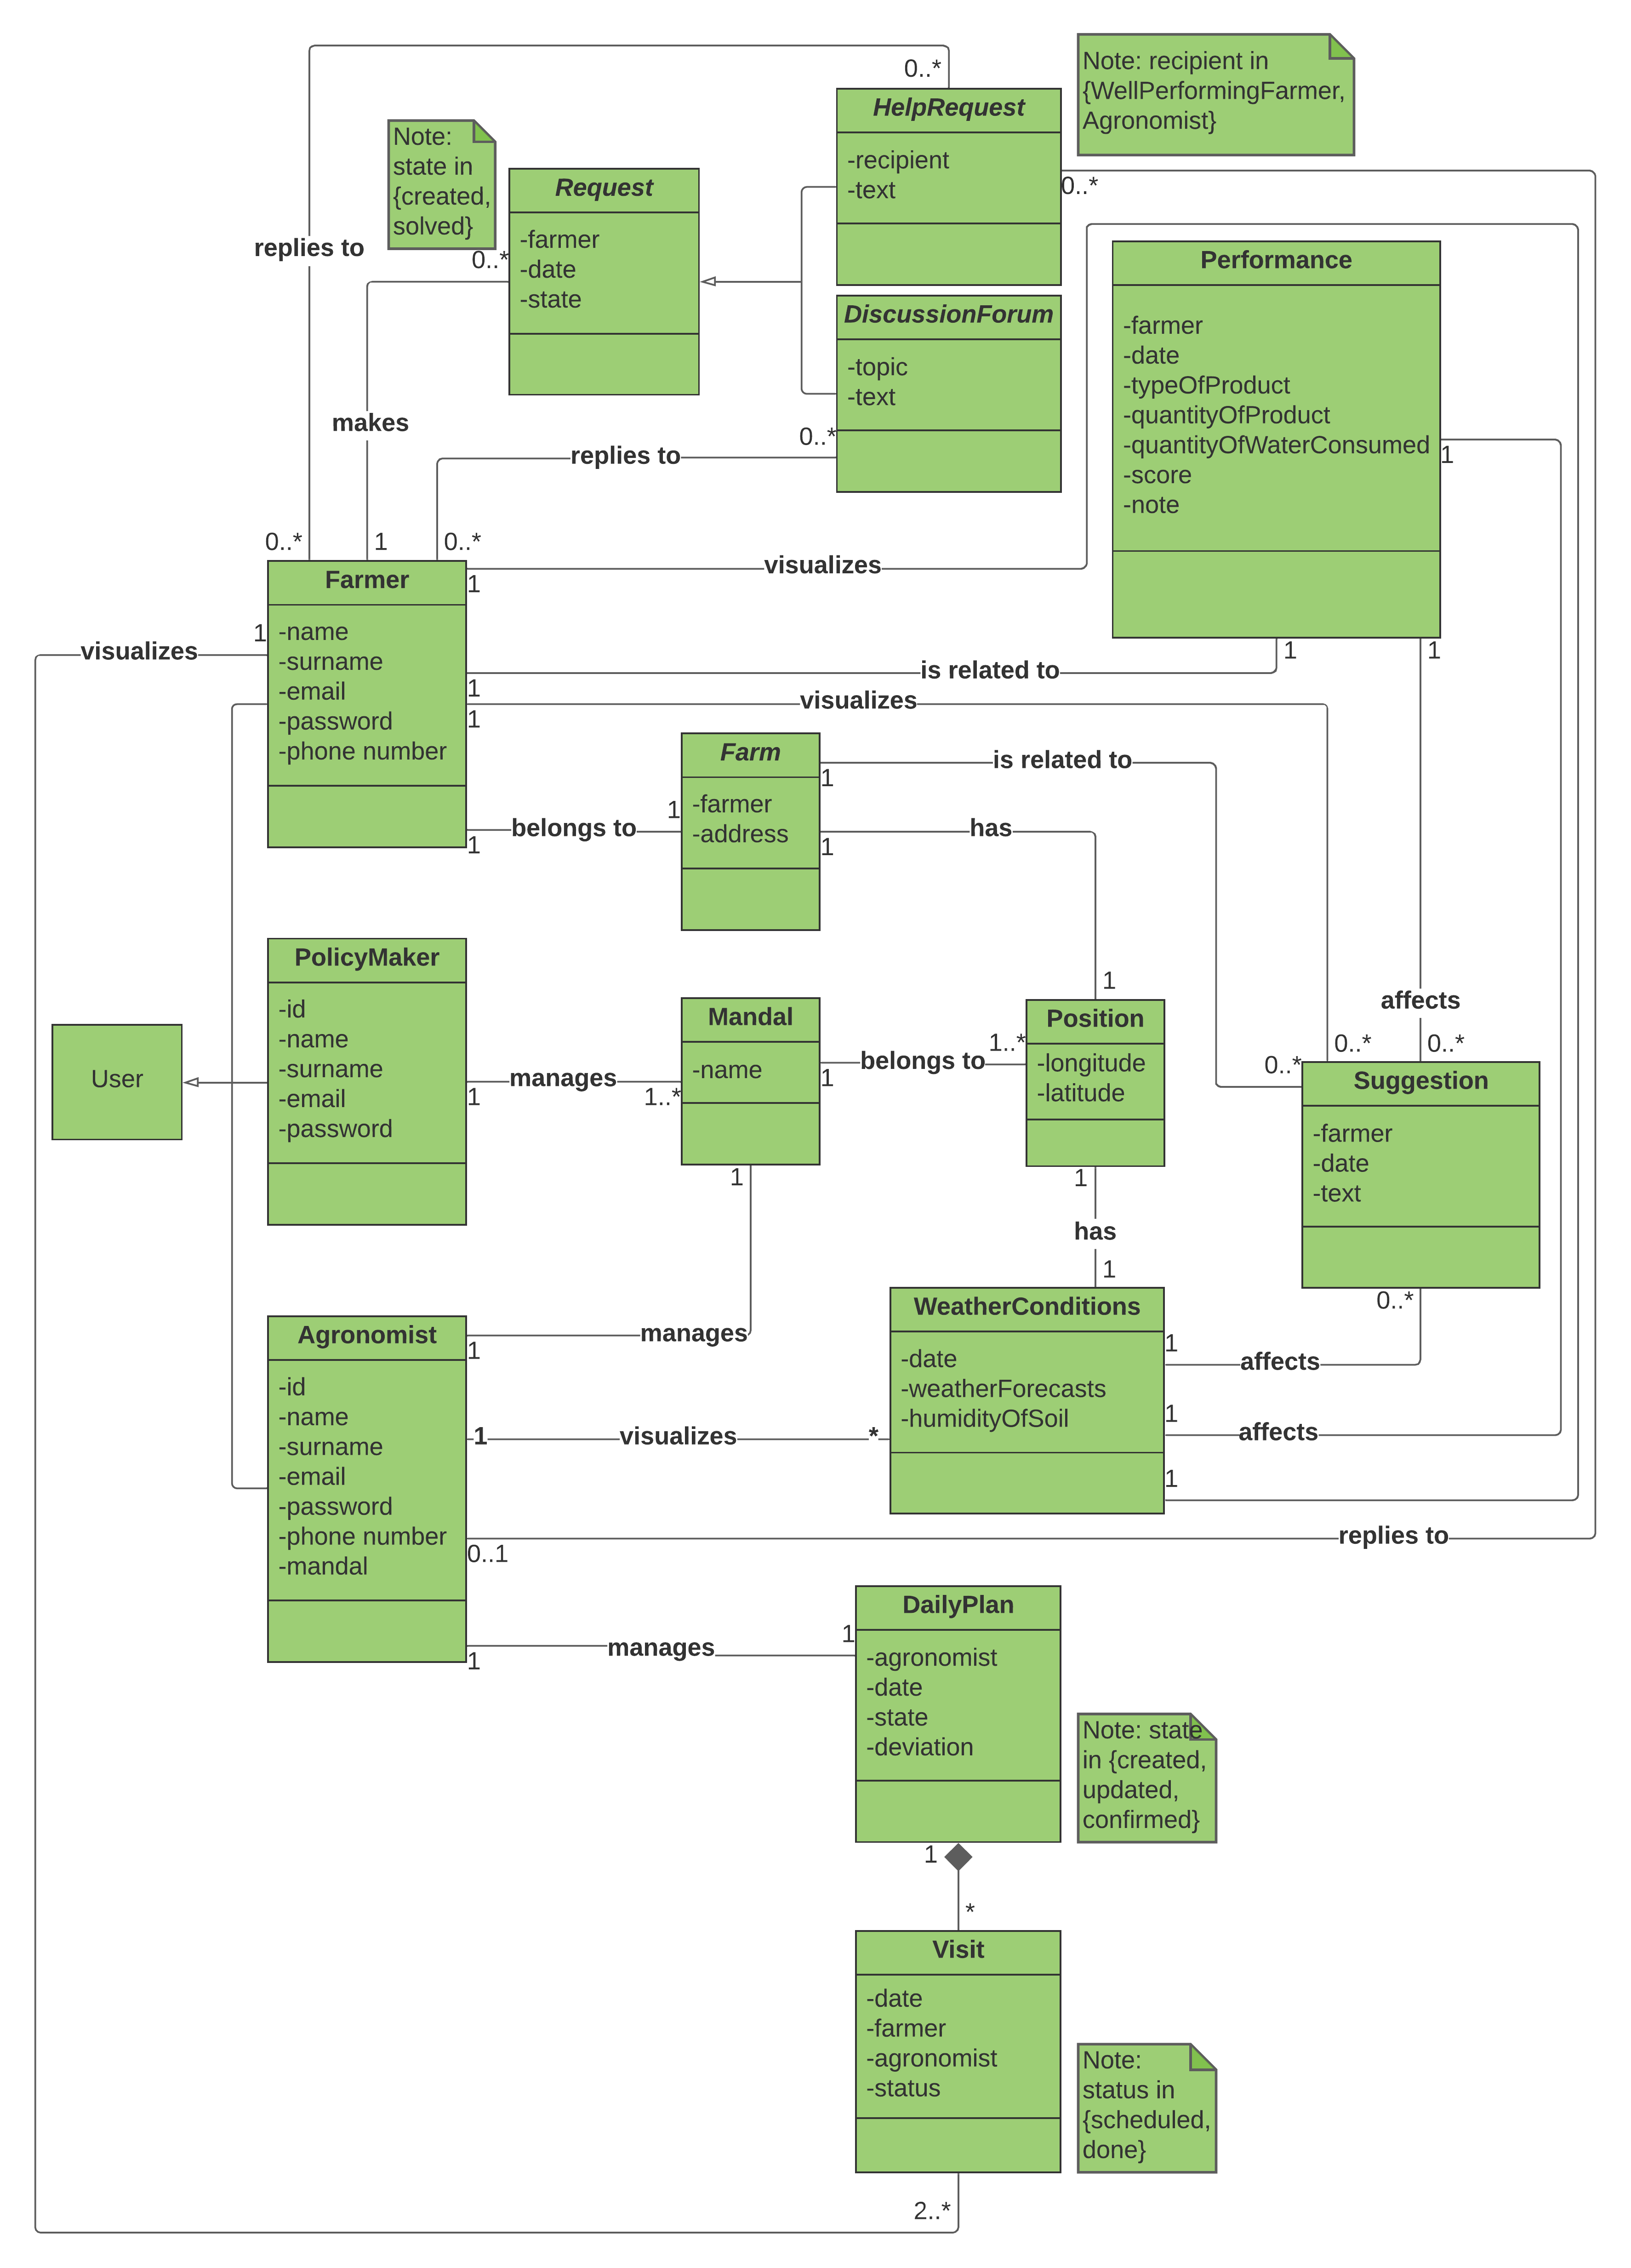
\includegraphics[width=125.5mm,scale=0.9]{./Images/Class Diagram DREAM.png}
  \caption{Class Diagram}
\end{figure}





\newpage



\subsection{State Charts}

\subsubsection{Daily Plan State Diagram}
This state diagram shows the three states of a Daily Plan.\\
The Daily Plan is \textit{Created} by the system and then \textit{Updated} or carried out and \textit{Confirmed} by the agronomist, depending on whether he needs to change the plan or not.
\begin{figure}[h!]
  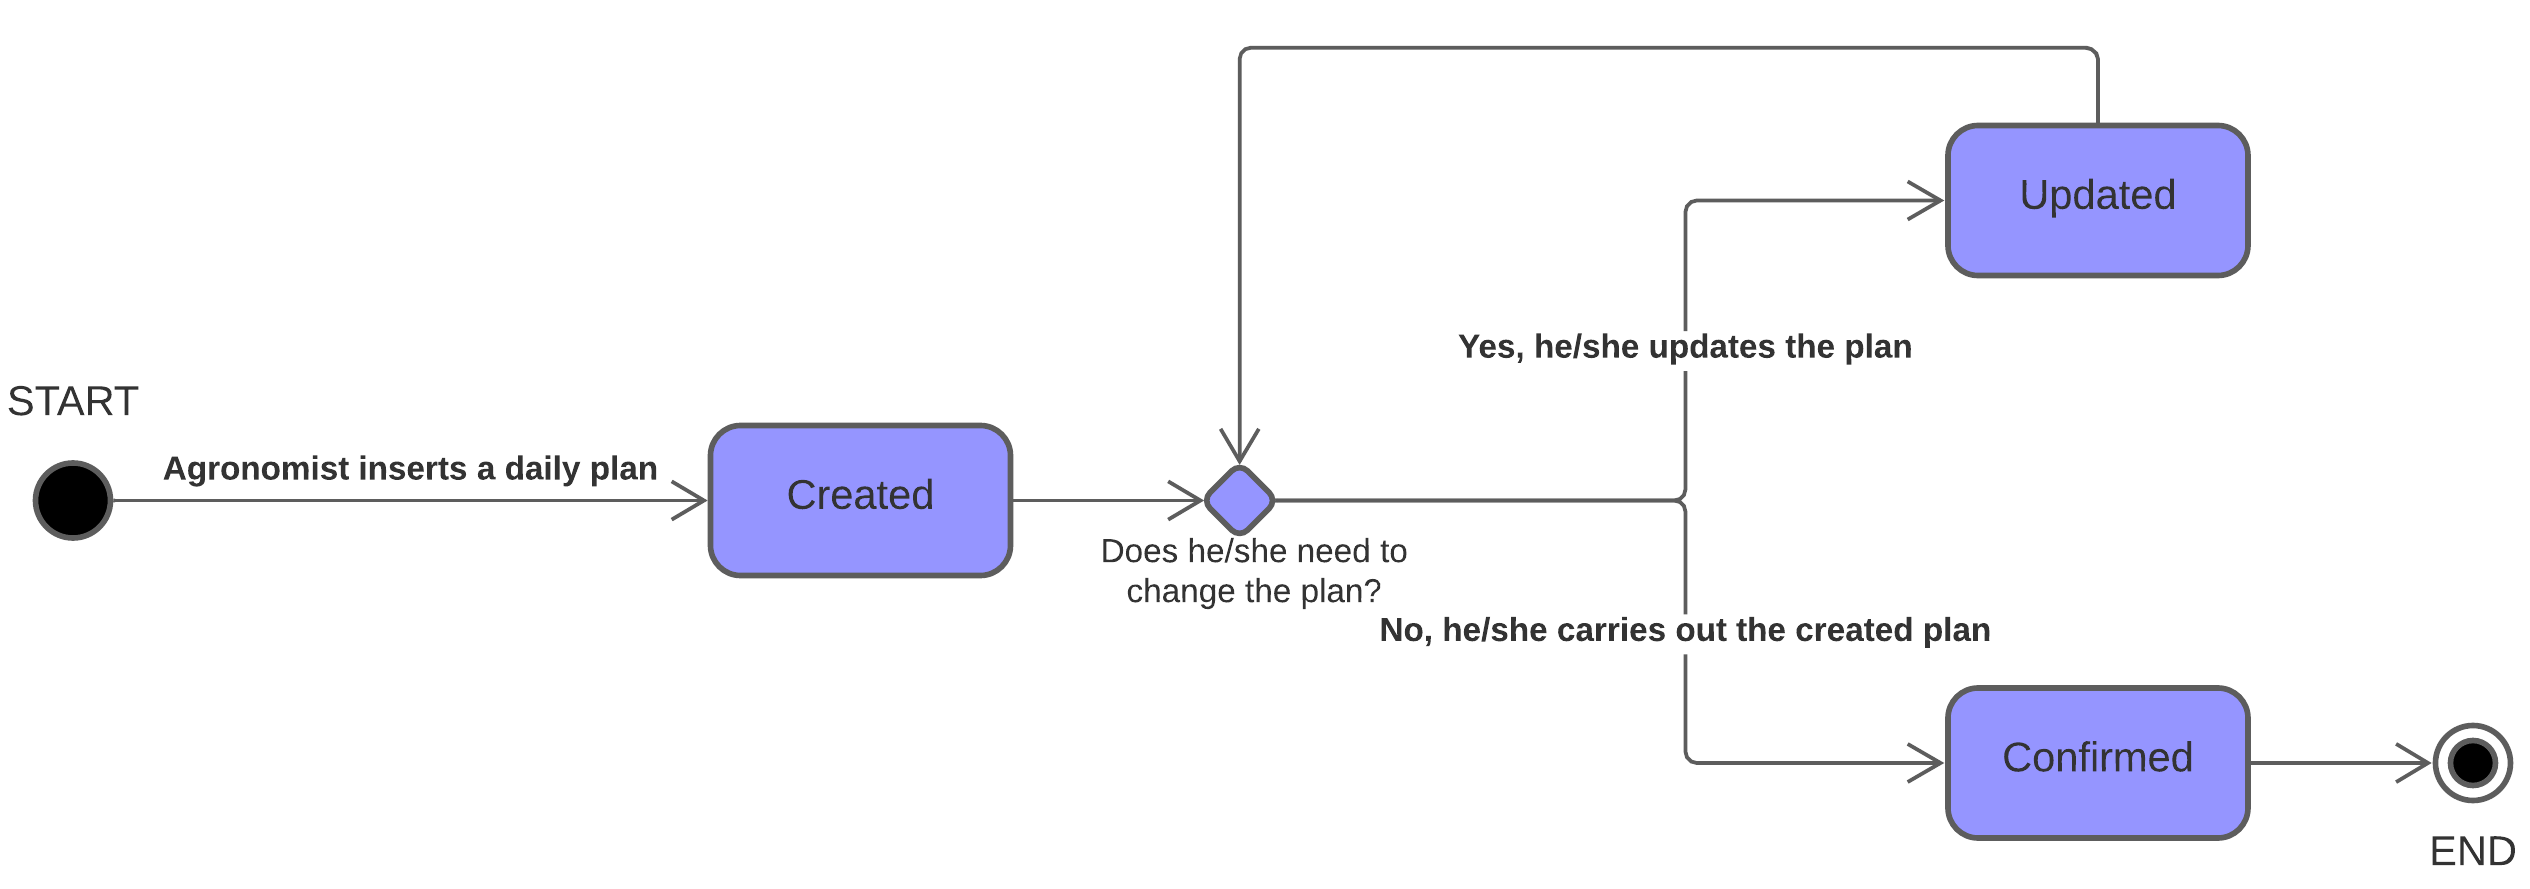
\includegraphics[width=\textwidth,height=\textheight,keepaspectratio]{./Images/State Chart DailyPlan.png}
  \caption{Daily Plan State Diagram}
\end{figure}

\subsubsection{Help Request State Diagram}
This state diagram shows the two states of a Help Request.\\
The Help Request is \textit{Created} and then \textit{Solved} by the farmer, depending on whether he is satisfied with the reply received or not.
\begin{figure}[h!]
  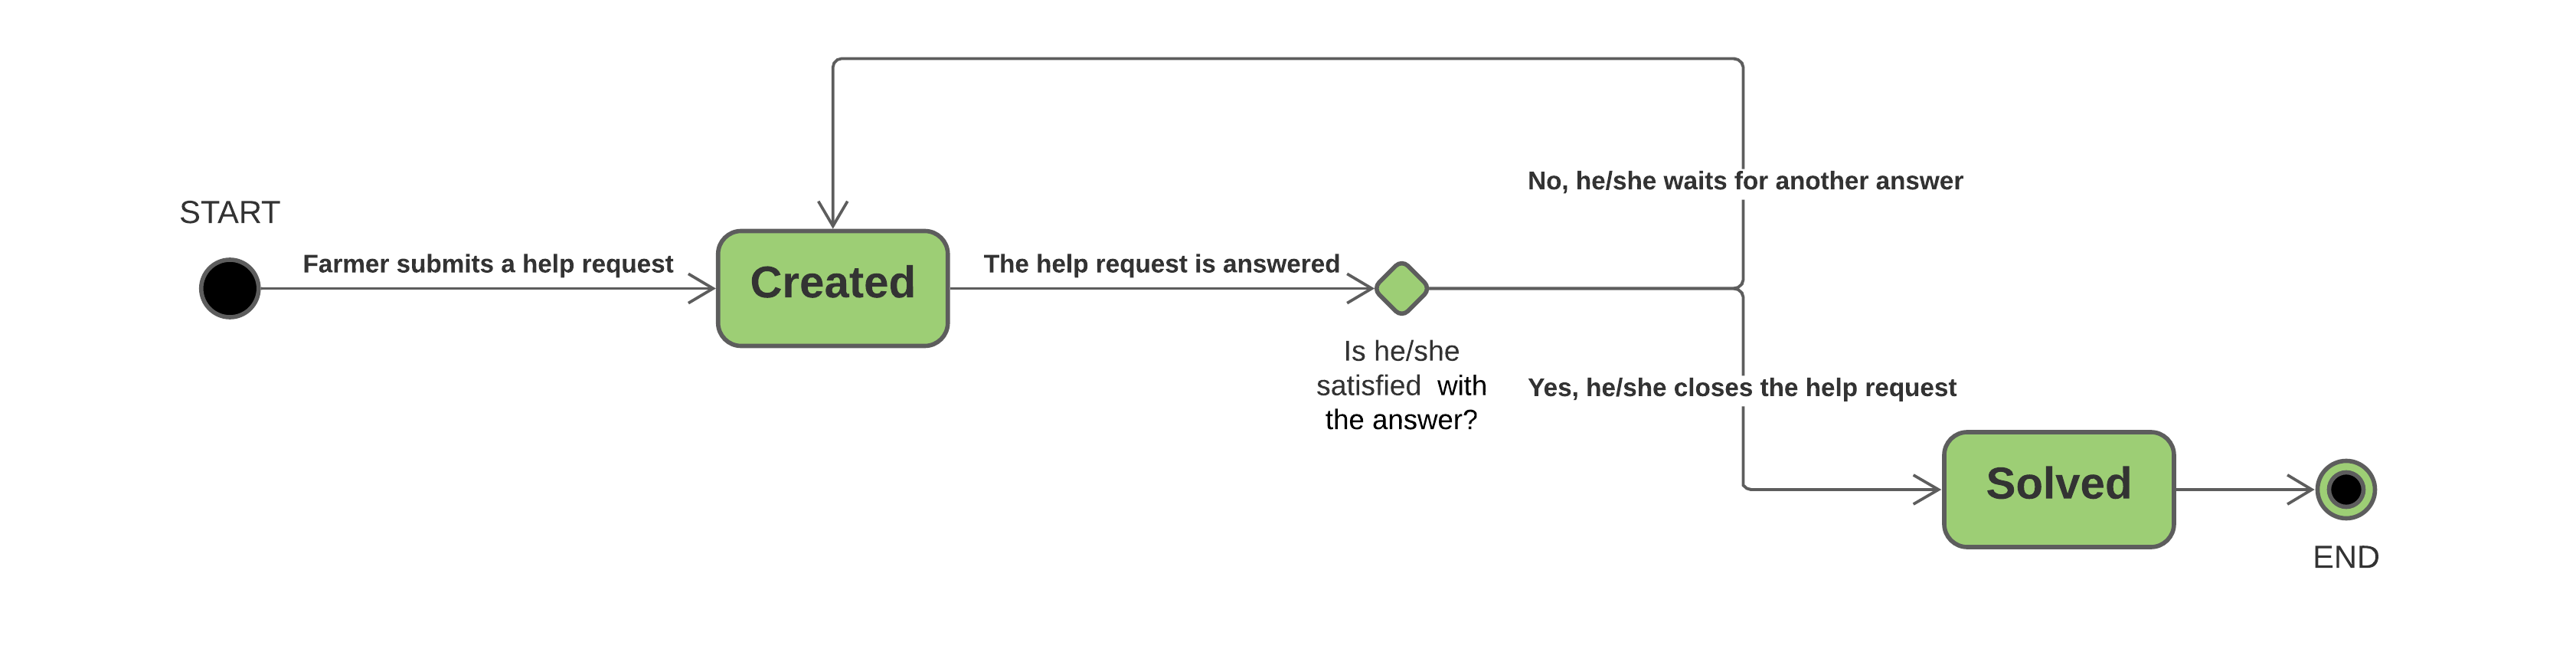
\includegraphics[width=\textwidth,height=\textheight,keepaspectratio]{./Images/State Chart HelpRequest.png}
  \caption{Help Request State Diagram}
\end{figure}

\subsubsection{Discussion Forum State Diagram}
This state diagram shows the two states of a Discussion Forum.\\
The Discussion Forum is \textit{Created} and then \textit{Solved} by the farmer, depending on whether he is satisfied with the replies received or not.
\begin{figure}[h!]
  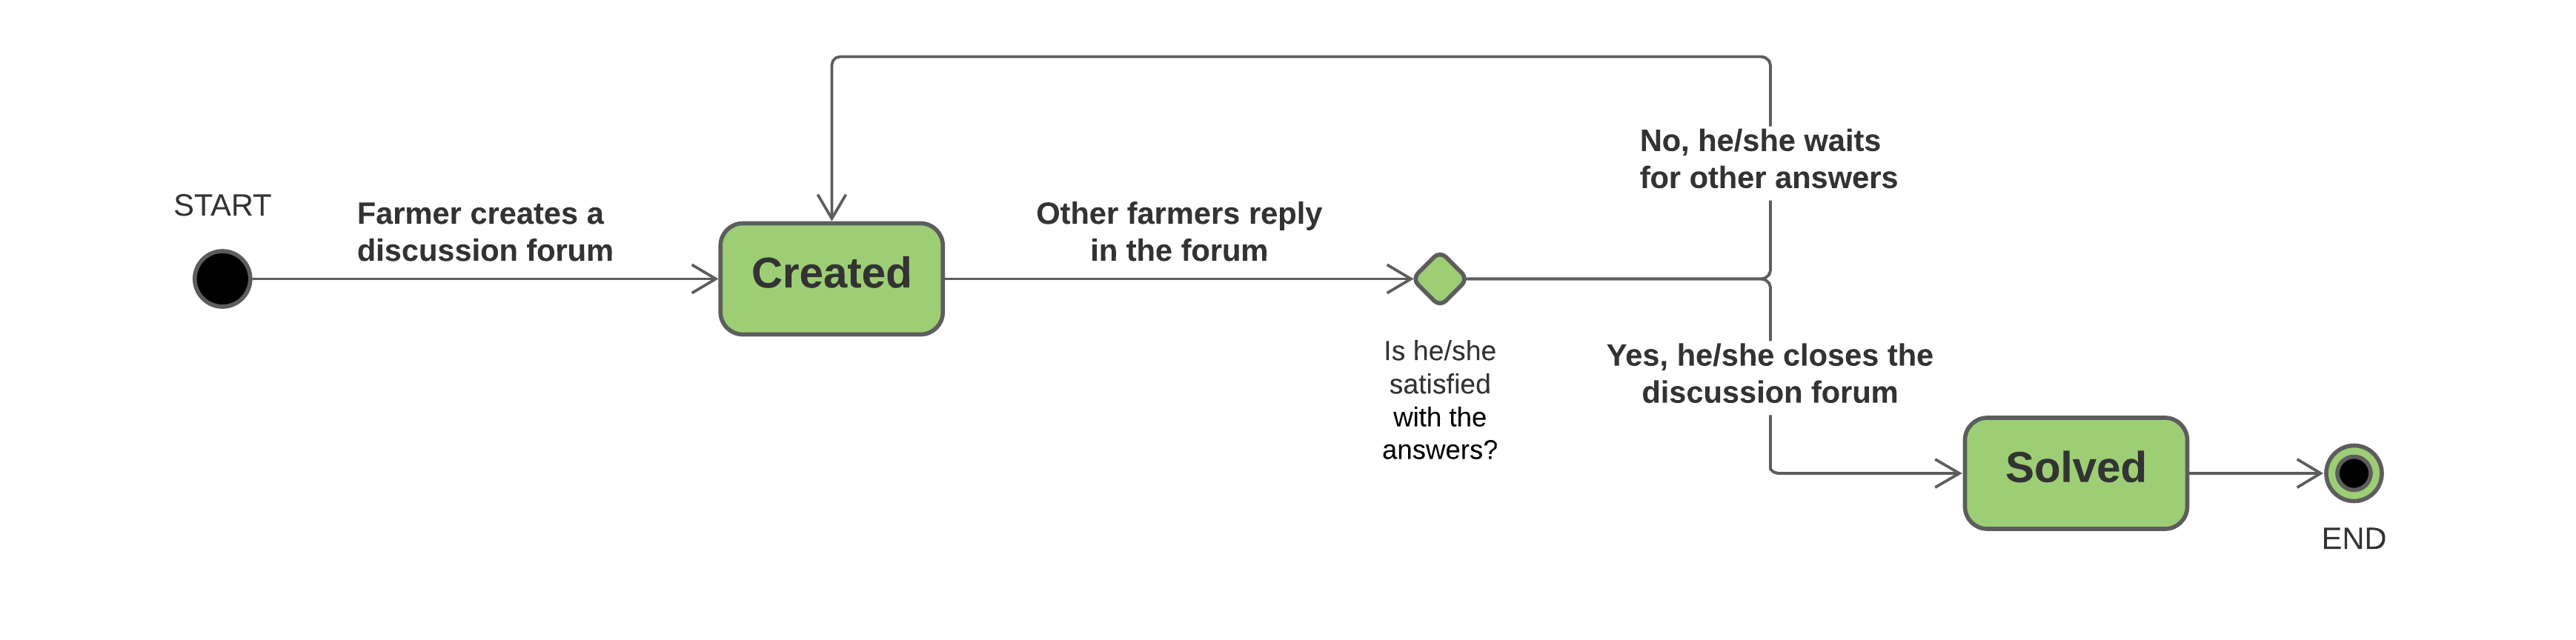
\includegraphics[width=\textwidth,height=\textheight,keepaspectratio]{./Images/State Chart DiscussionForum.png}
  \caption{Discussion Forum State Diagram}
\end{figure}

\subsubsection{Visit State Diagram}
This state diagram shows the two states of a Visit.\\
The Visit is \textit{Scheduled} and then \textit{Done} after the agronomist carries out the visit and confirms the corresponding Daily Plan.
\begin{figure}[h!]
  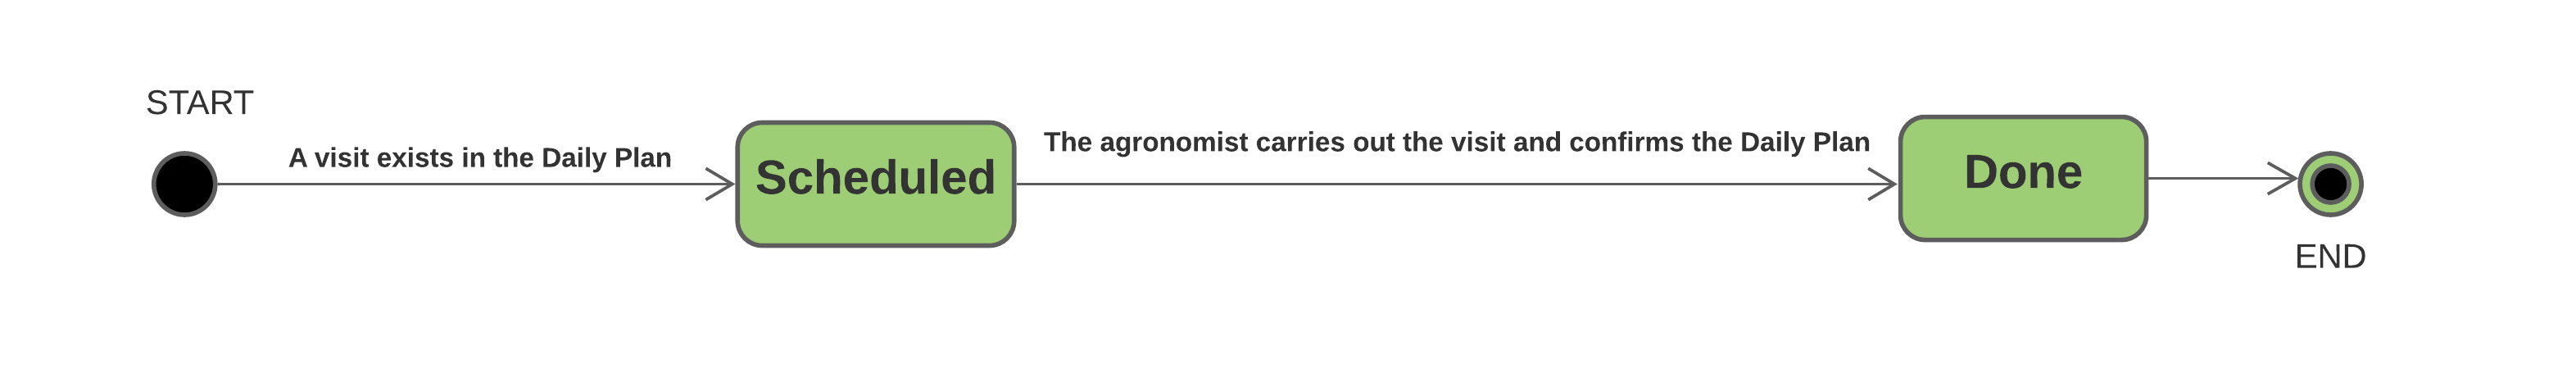
\includegraphics[width=\textwidth,height=\textheight,keepaspectratio]{./Images/State Chart Visit.png}
  \caption{Visit State Diagram}
\end{figure}

\section{Product functions}

\subsection{Registration}
In order to use the application all the actors (policy makers, agronomists and farmers) must be registered. The registration of an account can be performed in two ways: through the Web Application on a computer or through the mobile application on a smartphone.

In the case of the Web application, the farmer opens the web application and clicks on the "Register" button on the homepage. At this point he is redirected to the registration page where the farmer is asked to select which category of users he belongs to: "Policy Maker", "Farmer" or "Agronomist".
After selecting the right category he can enter in the predetermined fields the required data which in the case of the farmer are: name, surname, email, password, telephone number and his farm's address. The format of the characters entered is checked so that it complies with the predetermined rules of good formatting. 
If the rules on well-formed text are respected, a "Register now!" button appears. By clicking on it, the farmer is redirected to a new page that suggests to check his mailbox, where he will find an email generated and sent automatically by the system and with which the farmer can confirm his email by clicking on a link. After that the farmer is redirected to the login page in the Web app. The farmer then receives an email confirming his registration to DREAM.\\

Registration through the mobile application takes place in the same way as above. In fact, the farmer opens the application previously downloaded on his device. On the home page he clicks on the "Register" button. At this point he is redirected to the registration page where he can enter his data. The registration process continues as previously explained.\\

Registration takes place in the same way for all three actors, but there are some differences in the required data depending on the account role of the person who is registering. The data that agronomists and policy makers can enter are the same as those required by a farmer, with the exception of the farm's address.
The latter two roles (agronomists and policy makers) must enter an ID code assigned to them by the Telangana government to gain access to the system with their specific role after it is validated.
Moreover, only agronomists also have to inserts the mandal they are responsible of.


\subsection{Help Request}
DREAM allows farmers to make help request to the agronomist or even to well performing farmers if specified. The farmer accesses to the page "Help Request" and clicks on "Create a Help Request" button and accesses the corresponding page in which, in addition to the agronomist provided by default, he can select as recipient even well performing farmers of his/her same mandal. Eventually the farmer completes the text form corresponding to the body of the help request. Once finished, he/she confirms clicking on the correlated button "Confirm" and the help request is created. The help requests created by each farmer can be visualized by themselves accessing the page "Help Request" and clicking in the button "My Help Request". If someone replies the farmer visualizes in the same page the answer with the associated question \textit{"Are you satisfied with the answer?"} and the corresponding two possible answers \textit{"Yes"} or \textit{"No"}. Whether he/she is satisfied or not, he/she can:
\begin{enumerate}
    \item close the help request clicking on the button "Yes"
    \item not close it clicking on the button "No", waiting to receive other answers
\end{enumerate}
On the other hand, the users who can reply to a help request are the agronomist and well performing farmers of the same mandal. When a help request is created and they are mentioned among its recipients, they can visualize it in the "Help Request" page , where it is listed among the existing others. For each one there is a button "Answer" which they can click on to reply to the request.\\
Once the help request is solved by the farmer who made it, recipients cannot visualize it anymore. 

\subsection{Discussion Forum}
DREAM allows farmers to open a thread on the discussion forum. The farmer accesses the page "Discussion forum" and clicks on the button "Open a thread". He is redirected to a form which he fills in with topic and text and then he confirms. \\
The farmer can also look for a certain topic: he accesses the page "Discussion forum" and clicks on the button "Find a topic", the system provides him a form to fill in with the topic to be found and eventually it provides the farmer the list of existing associated threads.\\
If he wants to reply to one of them he can click on it and then, after pressing the button "Answer", he is redirected to a form in which he has to fill in the text's field. Eventually he confirms.

\subsection{Daily Plan}
DREAM allows agronomists to update the daily plan. He accesses the page "Daily Plan" and clicks on the button "Update". He is redirected to a form which he fills in with date (day and hour) and farmer and then he confirms. \\
The agronomist can also confirm the daily plan at the end of the day: he accesses the page "Daily Plan" and clicks on the button "confirm". He is redirected to a form with a field called "deviations" to be filled in only if modifications have been applied to the daily plan carried out during the day. Eventually he confirms.

\subsection{Notifications}
The system provides the farmer notifications regarding to: 
\begin{itemize}
    \item suggestions according to  his/her relevant information regarding his/her production and his/her farm's position
    \item new visits scheduled in the daily plan regarding him/her
    \item replies to his/her own help requests not yet solved
    \item replies to his/her own threads opened on the Discussion Forum
\end{itemize}
The agronomist and only well performing farmers are also provided with notifications regarding to new help requests received.\\

The actors involved can view the notification area directly from their homepage by clicking on the notification icon. At this point the actor is able to view all the notifications received in chronological order.

\subsection{Farmer inserts data regarding his production}
The farmer is allowed to enter relevant data about his production. Through his home page he has the possibility to insert new data on his harvest.
The data that the farmer has to enter in the form are: type of product and quantity of product collected. In addition, the farmer is allowed to add notes as well.\\
The system will add the current date of the insertion, the identification of the farmer (the email that uniquely identifies him) and the quantity of water consumed, information obtained thanks to some sensors.
After entering these data, the system will update the score for the farmer taking into account the new parameters entered.
The data entered will be saved in the database.


\section{Users Characteristics}
The actors of the applications are the following:
\begin{itemize}
    \item \textit {Policy maker}: he is an institutional figure in the public or private sector who has the power to elaborate and determine guidelines and strategies on the most relevant issues for society and politics. \textcolor{red}{He is registered into the application.}
    \item \textit {Agronomist}: he is a multidisciplinary professional figure. He works in favor of farms and small farmers by analyzing and developing projects based on direct observation and on the study of the best environmental solutions in order to improve productivity and enhance agricultural products. \textcolor{red}{He is registered into the application.}
    \item \textit {Farmer}: he is the figure who deals with managing, carrying out and producing crops of different kinds and types, constantly taking care of their good health. Furthermore, the farmer ensures that the places where the cultivation takes place fully comply with the hygienic-sanitary rules of the cultivation. They also provide for the maintenance of the structures necessary for the activities and the reclamation of the environments in which the cultivation takes place. \textcolor{red}{He is registered into the application.}
    \item \textit {Unregistered user}: a person who has not yet registered and is only allowed to sign up becoming either a Policy maker or an Agronomist or a Farmer depending on the type of membership.
\end{itemize}
\section{Assumptions, dependencies and constraints}

This subsection of the RASD lists each of the factors that affect the requirements stated in \textit{Chapter 3}.\\

An assumption is something that is believed to be true and which is outside of the project team’s control. Unlike constraints, which put restrictions on DREAM, assumptions open possibilities for it and make it possible its successful completion.
Eventually, dependencies refer to technology components, applications, and servers on which DREAM relies in order to be functional.

\subsection{Domain Assumptions}

\begin{itemize}
    \item [\textit{D.1}] Each user who wants to use the online service is needed to have a device connected to Internet 
    \item [\textit{D.2}] Data retrieved by external services (quantity of water consumed by each farmer, soil moisture and weather forecasts) are supposed to be accurate 
    \item [\textit{D.3}] A farmer does not forget to insert data regarding his production (type and quantity of product harvested)
    \item [\textit{D.4}] A farmer does not insert fraudulent information as input to  improve his performance score (e.g. higher quantity of product harvested)
    \item [\textit{D.5}] A farmer inserts in the system the correct address
    corresponding to his farm's location
    \item [\textit{D.6}] A help request is always solved
    \item [\textit{D.7}]The external service used by the system to retrieve latitude and longitude of a farm using the address provided by a farmer is supposed to be accurate
    \item [\textit{D.8}] A unique ID code is given to each policy maker to be able to register
    \item [\textit{D.9}] A unique ID code is given to each agronomist to be able to register
    \item [\textit{D.10}] ID codes assigned to policy makers and agronomists from Telangana government are collected in a database
    \item [\textit{D.11}] An agronomist inserts in the system the correct mandal he is responsible of
    \item [\textit{D.12}] An agronomist updates the daily plan when scheduling a new visit
    \item [\textit{D.13}] An agronomist confirms the daily plan specifying deviations correctly 
    \item [\textit{D.14}] An agronomist doesn't forget to confirm the daily plan by the end of the day
\end{itemize}


\subsection{Dependencies}

\begin{itemize}
    \item The system will exploit Internet connectivity of users' device
    \item The system will retrieve data collected in Telangana (water consumed by each farmer, soil moisture and weather forecasts) by external services
    \item The system will use an external service to compute latitude and longitude corresponding of a farm's address provided by a farmer
    \item The system will use an external service to check validity of ID code of policy makers and agronomist
\end{itemize}

\subsection{Constraints}

\subsubsection{Regulatory policies}
Access to confidential and sensitive data must be restricted to protect it from being lost or compromised in order to avoid adversely impacting users. At the same time, users must be able to access data as required for them to work effectively.\\ All sensitive data and user information are acquired by the company under the accepted terms and conditions. Telephone numbers and email addresses won't be used for commercial uses.

\subsubsection{Hardware limitations}
The system requires a compatible device (smartphone or personal computer) with Internet connection to work properly. 

\subsubsection{Interfaces to other applications}
The system relies on various external services to retrieve, compute and validate data needed for DREAM to work properly.

\subsubsection{Parallel operations}
Users of DREAM must be able to access DB at the same time, therefore parallel operations must be granted in order to avoid collision or any other integrity issue.


\chapter{Specific Requirements}

\section{External Interface Requirements}

In this section, most important user interfaces are shown.\\
Moreover, is given a description of the system in terms of hardware, 
software and communication interfaces.

\subsection{User Interfaces}

Vuoto
\subsection{Hardware Interfaces}

All actors requires a compatible device (smartphone or personal computer) with Internet connection to allow DREAM to work properly.\\
In particular, policy makers should access the application using a computer to maximize their experience while farmers should prefer to use a smartphone. Eventually agronomist must use both computer and smartphone using the application according to the functionalities they need to exploit.
\subsection{Software Interfaces}

The system relies on various external services accessible through API to compute and retrieve near-real time data:
\begin{itemize}
    \item \textit{Maps Service} to retrieve the position (latitude and longitude) of farms' address inserted by farmers
    \item \textit{Copernicus Climate Data Store Service} to retrieve data regarding soil moisture
    \item \textit{Telangana Government Service} to retrieve weather forecasts
    \item \textit{Telangana Water Irrigation System Service} to retrieve the amount of water consumed by each farmer
\end{itemize}
It also accesses ID codes’ DB managed by Telangana government to check validity of ID code inserted by policy makers and agronomist while registering into DREAM.


\subsection{Communication Interfaces}

All devices used by actors are connected to the system through Internet connection.
\section{Functional Requirements}

Functional requirements capture the intended behavior of the system and are derived through Use Cases.\\
A use case defines a goal-oriented set of interactions between external actors and the system under consideration. 

\subsection{Use Case Diagrams}
\begin{center}
\begin{figure}[H]
  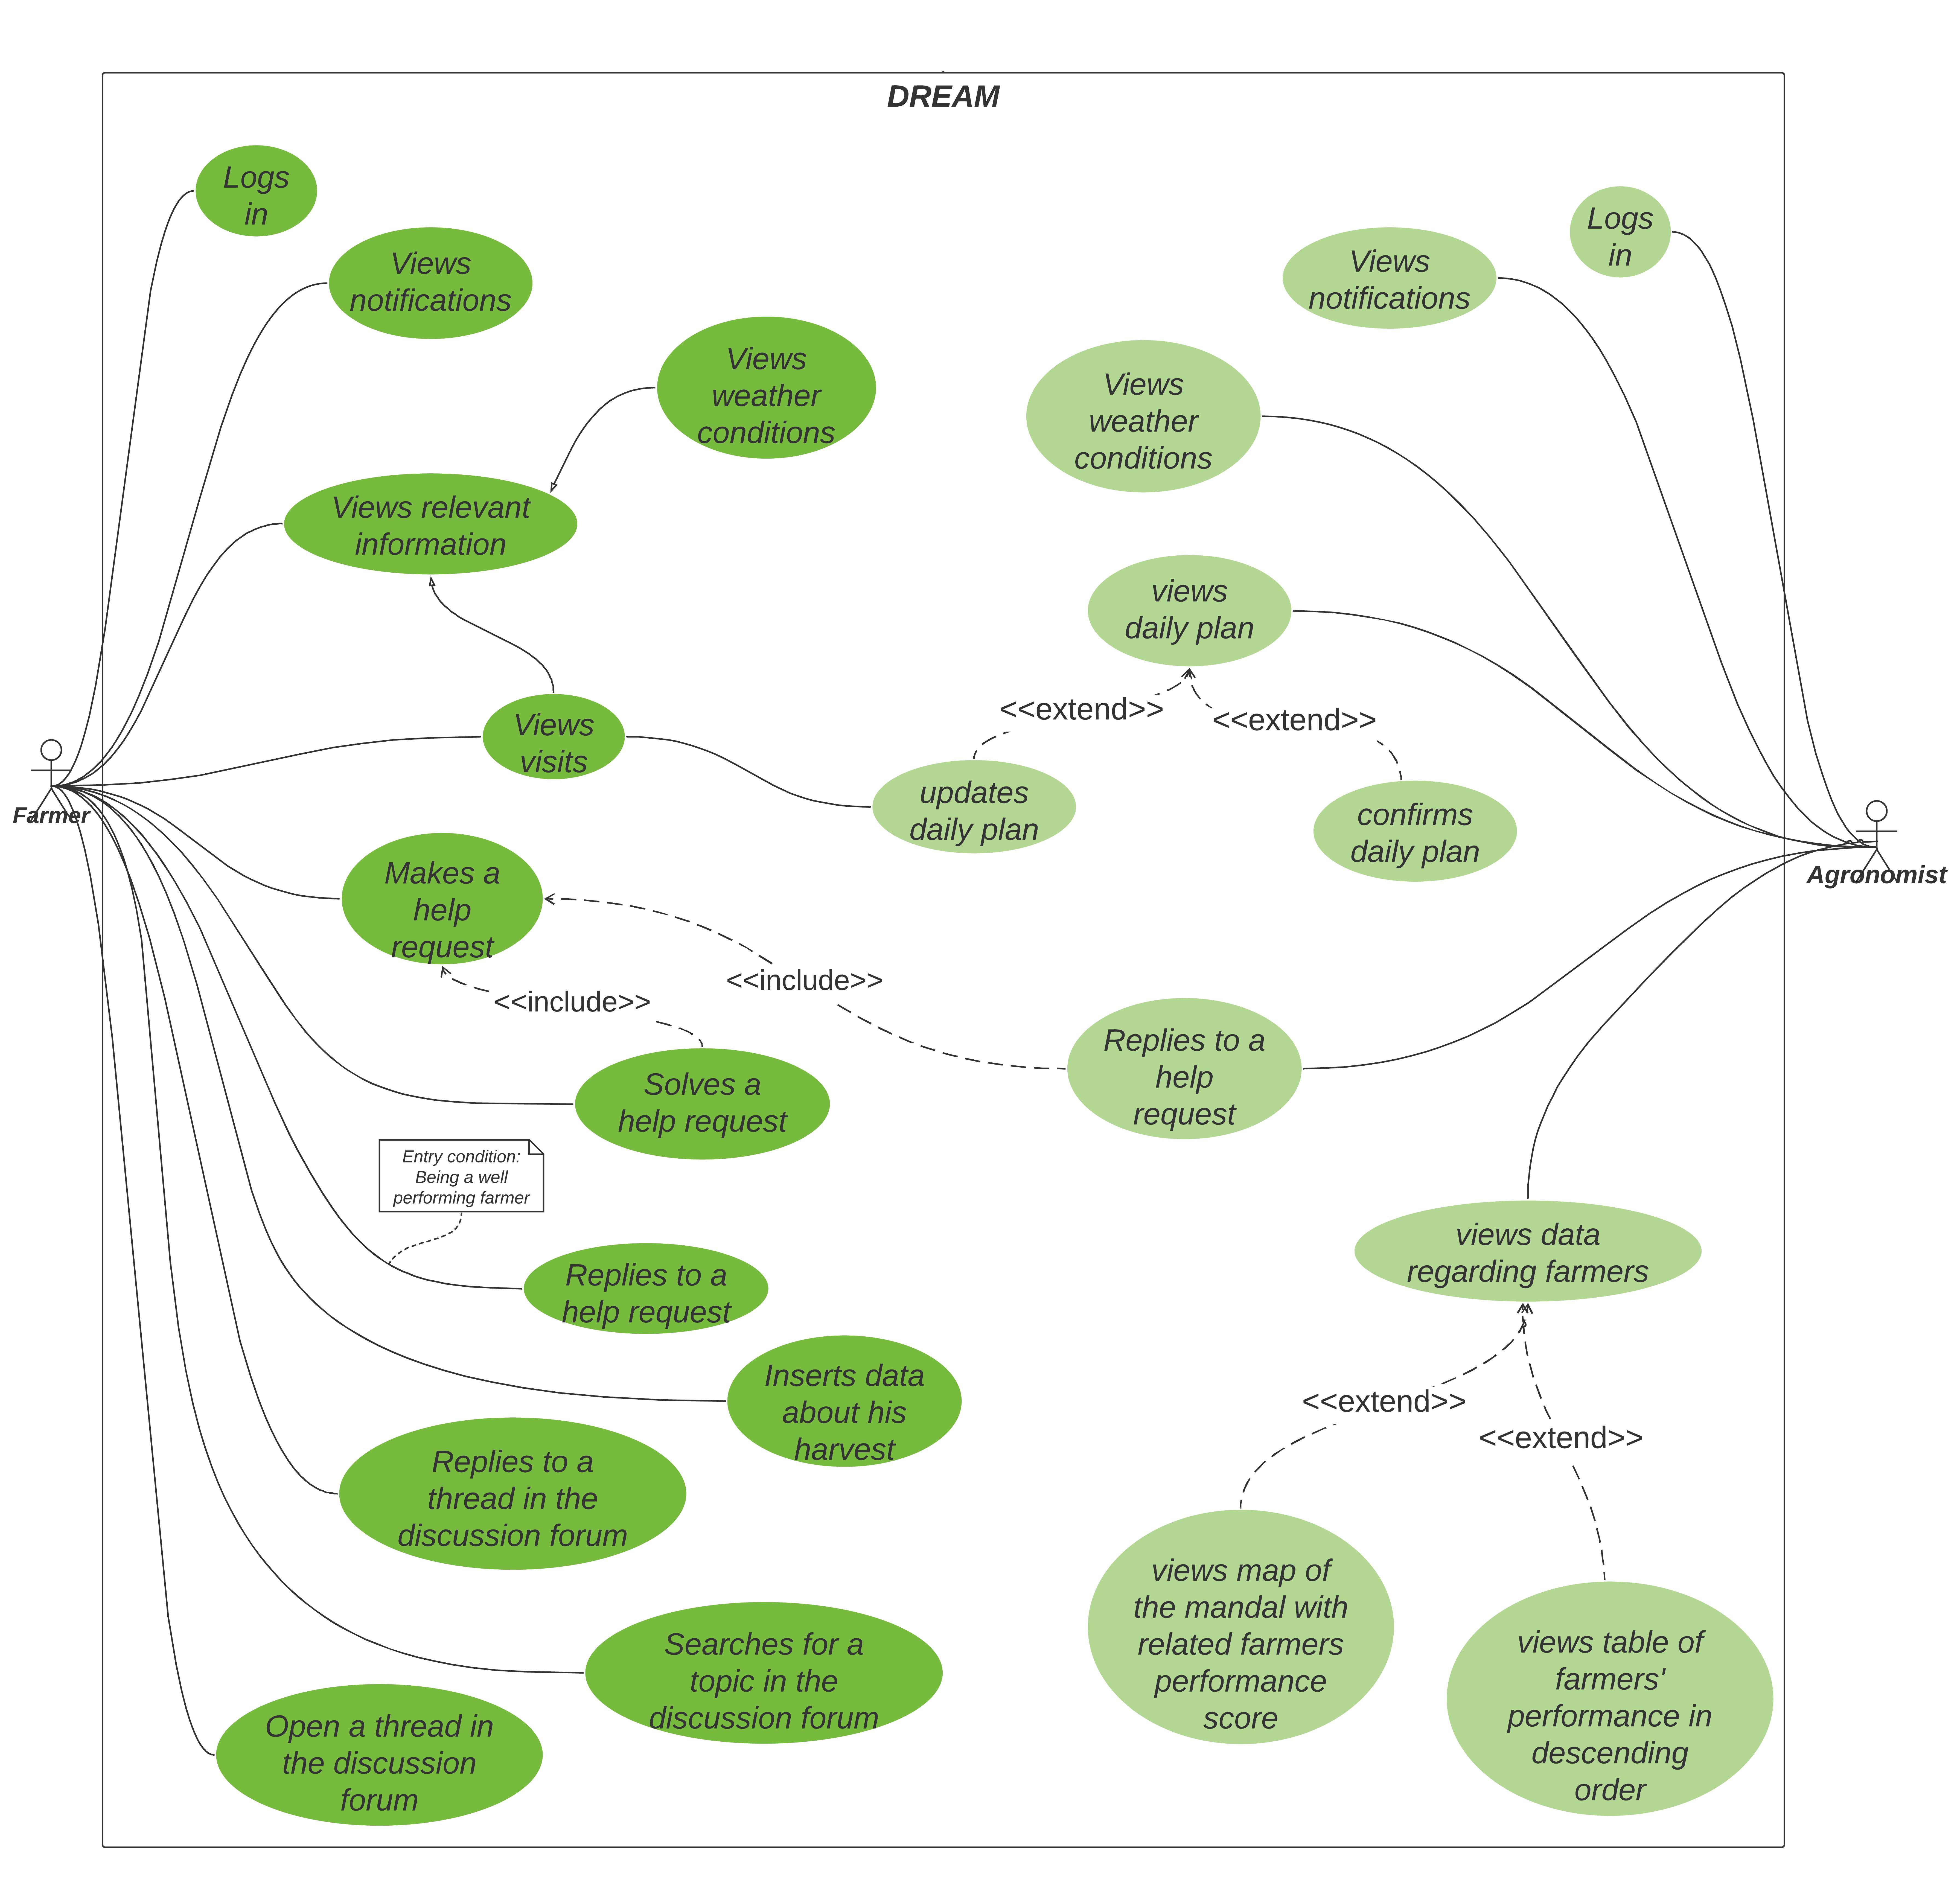
\includegraphics[width=\textwidth,height=\textheight,keepaspectratio]{./Images/Use case Agronomist Farmer.png}
  \caption{Use Case Diagram - Farmer and agronomist}
\end{figure}

\begin{figure}[H]
  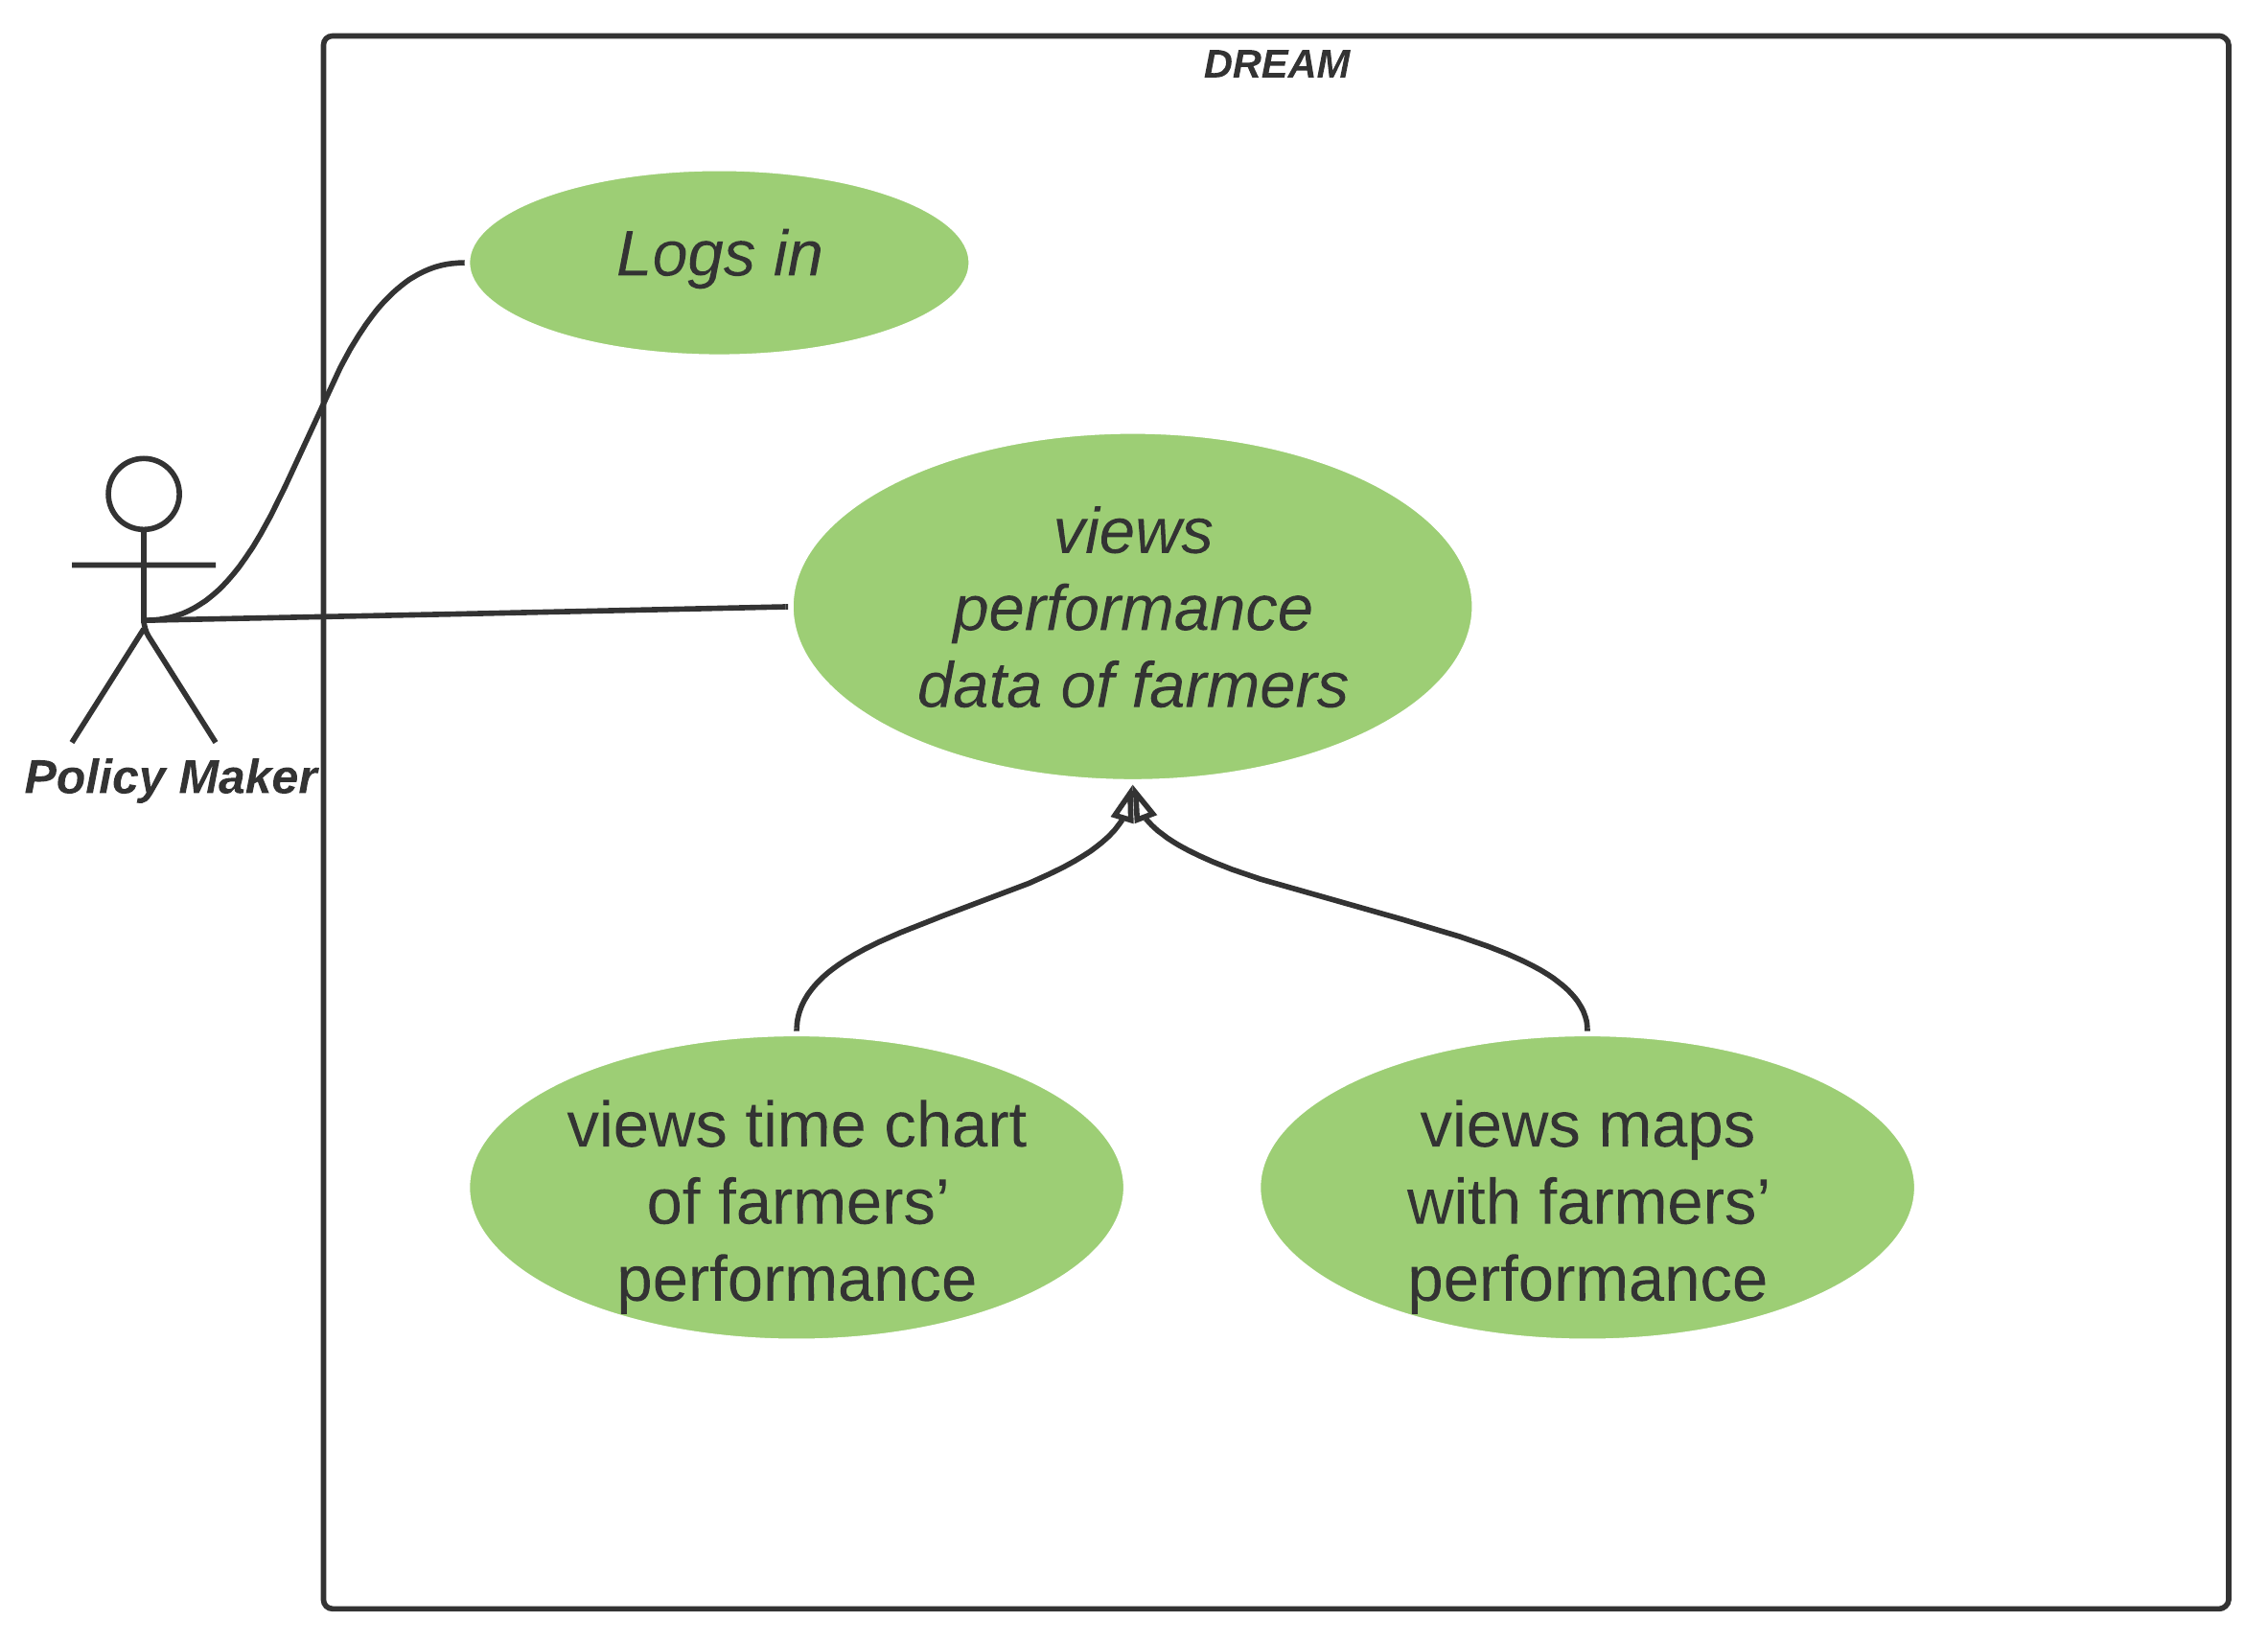
\includegraphics[width=\textwidth,height=\textheight,keepaspectratio]{./Images/Use case Policy Maker.png}
  \caption{Use Case Diagram - Policy maker}
\end{figure}
\end{center}

\subsection{Use Case Analysis}
\begin{center}

\setlist[enumerate]{leftmargin=*,noitemsep, topsep=3pt}
\setlist[itemize]{leftmargin=*,noitemsep, topsep=3pt}
\setlength\tabcolsep{5pt}
\renewcommand{\arraystretch}{1.5}

\begin{table}[H]
\begin{tabular}{|m{1.8cm}|m{10cm}|} 
  \hline
  \footnotesize{\textbf{Name}} & UC.1 \textit{Unregistered user registers into the application}\\
  \hline
  \footnotesize{\textbf{Actors}} & Unregistered user\\ 
  \hline
  \footnotesize{\textbf{Entry \newline{conditions}}} & Unregistered user wants to join DREAM\\
  \hline
  \footnotesize{\textbf{Flow \newline{of events}}} &
  \begin{enumerate}
      \item The unregistered User accesses the \textit{Registration} page on the application.
      \item The unregistered user selects which category of users he belongs to: "Policy Maker", "Farmer" or "Agronomist".
      \item The system provides the user with the appropriate form to fill.
      \item The unregistered user fills in all the mandatory fields.
      \item The system let "Register now!" button appear.
      \item The unregistered user clicks on the "Register now!" button.
      \item The system saves data of the new user.
      \item The system sends an email to the new user.
      \item The user is redirected on a waiting page that suggests him to check his mailbox.
      \item The user confirms his email by clicking on the link in the email within ten minutes.
      \item The user is redirected to the \textit{Login} page.
      \vspace*{-\baselineskip}
  \end{enumerate}
  \vspace*{-\baselineskip}\\
  \hline
  \footnotesize{\textbf{Exit \newline{conditions}}} & The unregistered user successfully ends the registration process and he becomes new user.\\
  \hline
  \footnotesize{\textbf{Exceptions}} & 
  \begin{enumerate}
      \item The unregistered user inserts invalid information in the fields.
      \item The unregistered user does not fill in all the required fields.
      \item The unregistered user inserts a username that is not available.
      \item The user does not confirm his email by clicking on the link within ten minutes.
  \end{enumerate}
  Exceptions 1 to 3 are handled by not making the "Register now!" button appear and activating an alert message that invites the user to double-check the data entered.\\
  \hline
\end{tabular}
\end{table}

\begin{table}[H]

\begin{tabular}{|m{1.8cm}|m{10cm}|} 
  \hline
  \footnotesize{\textbf{Name}} & UC.2 \textit{User logs in the application}\\
  \hline
  \footnotesize{\textbf{Actors}} & Farmer / Agronomist / Policy maker\\ 
  \hline
  \footnotesize{\textbf{Entry \newline{conditions}}} & The user has already registered.\\
  \hline
  \footnotesize{\textbf{Flow \newline{of events}}} & 
  \begin{enumerate}
      \item The user opens the \textit{Login} page.
      \item The user inserts his username.
      \item The user inserts his password.
      \item The user click on the "Login" button.
      \item The system checks that the parameters entered correspond to those of a registered account.
      \item The user is redirected to his \textit{Home} page.
      \vspace*{-\baselineskip}
  \end{enumerate}\\
  \hline
  \footnotesize{\textbf{Exit \newline{conditions}}} & The user successfully logs in and he is identified with the role (Farmer / Agronomist / Policy maker) with which he was previously registered.\\
  \hline
  \footnotesize{\textbf{Exceptions}} & 
 \begin{enumerate}
      \item The user did not fill in both required fields.
      \item The user has filled in one or both fields incorrectly.
      \vspace*{-\baselineskip}
  \end{enumerate}\\
  \hline
\end{tabular}
\end{table}

\begin{table}[H]
\begin{tabular}{|m{1.8cm}|m{10cm}|} 
  \hline
  \footnotesize{\textbf{Name}} & UC.3 \textit{Farmer inserts data about product harvested into the application}\\
  \hline
  \footnotesize{\textbf{Actors}} & Farmer\\ 
  \hline
  \footnotesize{\textbf{Entry \newline{conditions}}} & Farmer has already logged in.\\
  \hline
  \footnotesize{\textbf{Flow \newline{of events}}} &
  \begin{enumerate}
      \item The farmer clicks on the "+" button on his \textit{Home} page.
      \item The system shows a new form to fill out.
      \item The farmer inserts the type of product of his harvest.
      \item The farmer inserts the quantity of product of his harvest.
      \item The farmer inserts notes about his harvest.
      \item The farmer clicks on the "Add" button.
      \item The system adds the parameter "username" of the farmer to the request.
      \item The system adds the parameter "current date" to the request.
      \item The system adds the parameter "quantity of water consumed" to the request.
      \item The system inserts the data in the database.
      \item The system refresh the \textit{Home} page.
      \item The system returns a message that the information has been added.
      \vspace*{-\baselineskip}
  \end{enumerate}\\
  \hline
  \footnotesize{\textbf{Exit \newline{conditions}}} & 
  \begin{itemize}
      \item The farmer has successfully inserted his harvest information.
      \item The farmer received the confirmation message for adding data on his crop.
      \vspace*{-\baselineskip}
  \end{itemize}\\
   \hline
  \footnotesize{\textbf{Exceptions}} & 
 \begin{enumerate}
      \item The inserted data are not well formatted.
      \item Sensor data are not available at the moment.
      \vspace*{-\baselineskip}
  \end{enumerate}\\
  \hline
\end{tabular}
\end{table}

\begin{table}[H]
\begin{tabular}{|m{1.8cm}|m{10cm}|} 
  \hline
  \footnotesize{\textbf{Name}} & UC.4 \textit{Farmer makes a help request}\\
  \hline
  \footnotesize{\textbf{Actors}} & Farmer\\ 
  \hline
  \footnotesize{\textbf{Entry \newline{conditions}}} & Farmer has already logged in.\\
  \hline
  \footnotesize{\textbf{Flow \newline{of events}}} & 
  \begin{enumerate}
      \item The farmer accesses the \textit{Help request} page by clicking on the appropriate icon on the \textit{Home} page.
      \item The farmer clicks on the "Create Help Request" button.
      \item By default the system adds the responsible agronomist to the recipients of the help request.
      \item The farmer add to the recipient list well performing farmers.
      \item The farmer writes the help request in the appropriate field.
      \item The farmer clicks on the "Confirm" button.
      \item The system adds the parameter "username" of the farmer to the request.
      \item The system adds the parameter "current date" to the request.
      \item The system inserts the data in the database.
      \item The system updates the \textit{Help Request} page.
      \item The system returns a message that the help request has been created.
      \vspace*{-\baselineskip}
  \end{enumerate}\\
  \hline
  \footnotesize{\textbf{Exit \newline{conditions}}} & The farmer has successfully send a help request.\\
  \hline
  \footnotesize{\textbf{Exceptions}} & There are no well performing farmers in his mandal.\\
  \hline
\end{tabular}
\end{table}

\begin{table}[H]
\begin{tabular}{|m{1.8cm}|m{10cm}|} 
  \hline
  \footnotesize{\textbf{Name}} & UC.5 \textit{Farmer solves a help request}\\
  \hline
  \footnotesize{\textbf{Actors}} & Farmer\\ 
  \hline
  \footnotesize{\textbf{Entry \newline{conditions}}} & Farmer has already logged in and he has  previously created a help request that is not yet marked as solved.\\
  \hline
  \footnotesize{\textbf{Flow \newline{of events}}} & 
  \begin{enumerate}
      \item The farmer accesses the \textit{Help Request} page by clicking on the appropriate icon on the \textit{Home} page.
      \item The farmer visualize his help requests by clicking on "My Help Request" button.
      \item The system shows the list of all the help requests of the farmer created, but not solved.
      \item The system shows two answer buttons "yes" or "no" to the question "Are you satisfied with the answer?" when the farmer receives a response to a help request.
      \item The farmer closes the request for help by declaring that he is satisfied with the answer received by clicking on the "yes" button.
      \item The system updates the status of the response to solved in the database.
      \item The system updates the \textit{Help Request} page.
      \item The system returns a message that the help request has been solved.
      \vspace*{-\baselineskip}
  \end{enumerate}\\
  \hline
  \footnotesize{\textbf{Exit \newline{conditions}}} & The farmer has successfully solved a help request.\\
  \hline
  \footnotesize{\textbf{Exceptions}} & 
 \begin{enumerate}
      \item There are no farmer help requests created, but not solved.
      \item No one has yet replied to the farmer's help request.
      \vspace*{-\baselineskip}
  \end{enumerate}\\
  \hline
\end{tabular}
\end{table}

\begin{table}[H]
\begin{tabular}{|m{1.8cm}|m{10cm}|} 
  \hline
  \footnotesize{\textbf{Name}} & UC.6 \textit{Farmer searches for a topic on the discussion forum}\\
  \hline
  \footnotesize{\textbf{Actors}} & Farmer\\ 
  \hline
  \footnotesize{\textbf{Entry \newline{conditions}}} & Farmer has already logged in\\
  \hline
  \footnotesize{\textbf{Flow \newline{of events}}} & 
  \begin{enumerate}
      \item The farmer accesses the \textit{Discussion Forum} page by clicking on the appropriate icon on the \textit{Home} page.
      \item The farmer clicks on the "Find a topic" button.
      \item The system shows a form to be filled in with the mandatory field \textit{topic}.
      \item The farmer inserts the topic to be found.
      \item The farmer confirms by clicking on the corresponding button.
      \vspace*{-\baselineskip}
  \end{enumerate}\\
  \hline
  \footnotesize{\textbf{Exit \newline{conditions}}} & The system provides the farmer a list with all associated threads already existing on the discussion forum.\\
  \hline
  \footnotesize{\textbf{Exceptions}} & 
 \begin{enumerate}
      \item There are no existing threads related to a certain topic on the discussion forum. In this case, the system suggests to attempt a new research or to open a new thread.
      \item The farmer does not fill out the form with the mandatory data.
      \vspace*{-\baselineskip}
  \end{enumerate}\\
  \hline
\end{tabular}
\end{table}

\begin{table}[H]
\begin{tabular}{|m{1.8cm}|m{10cm}|}  
  \hline
  \footnotesize{\textbf{Name}} & UC.7 \textit{Farmer opens a thread on the discussion forum}\\
  \hline
  \footnotesize{\textbf{Actors}} & Farmer\\ 
  \hline
  \footnotesize{\textbf{Entry \newline{conditions}}} & Farmer has already logged in.\\
  \hline
  \footnotesize{\textbf{Flow \newline{of events}}} & 
  \begin{enumerate}
      \item The farmer accesses the \textit{Discussion Forum} page by clicking on the appropriate icon on the \textit{Home} page.
      \item The farmer clicks on the "Open a thread" button.
      \item The system shows a form to be filled in with the the mandatory fields \textit{topic} and \textit{text}.
      \item The farmer inserts mandatory data.
      \item The farmer confirms by clicking on the corresponding button.
      \item The system updates the \textit{Discussion Forum} page.
      \item The system returns a message that the thread has been created on the discussion forum.
      \vspace*{-\baselineskip}
  \end{enumerate}\\
  \hline
  \footnotesize{\textbf{Exit \newline{conditions}}} & The farmer has successfully opened a new thread.\\
  \hline
  \footnotesize{\textbf{Exceptions}} & The farmer does not fill out the form with the mandatory data.\\
  \hline
\end{tabular}
\end{table}

\begin{table}[H]
\begin{tabular}{|m{1.8cm}|m{10cm}|} 
  \hline
  \footnotesize{\textbf{Name}} & UC.8 \textit{Farmer replies on the discussion forum}\\
  \hline
  \footnotesize{\textbf{Actors}} & Farmer\\ 
  \hline
  \footnotesize{\textbf{Entry \newline{conditions}}} & Farmer has already logged in.\\
  \hline
  \footnotesize{\textbf{Flow \newline{of events}}} & 
  \begin{enumerate}
      \item The farmer accesses the \textit{Discussion Forum} page by clicking on the appropriate icon on the \textit{Home} page.
      \item The system shows a list of existing threads only visualizing the associated topic.
      \item The farmer clicks on a certain thread.
      \item The farmer visualizes its details and all the correlated answers already received.
      \item The farmer clicks on the button "Reply".
      \item The system shows a form to be filled in with the mandatory field \textit{text}.
      \item The farmer inserts mandatory data.
      \item The farmer confirms by clicking on the corresponding button.
      \item The system associates the response of the farmer to the thread on the discussion forum.
      \item The system updates the thread page.
      \item The system returns a message that the farmer has successfully answered to a thread on the discussion forum.
      \vspace*{-\baselineskip}
  \end{enumerate}\\
  \hline
  \footnotesize{\textbf{Exit \newline{conditions}}} & The farmer has successfully answered to a thread on the discussion forum.\\
  \hline 
  \footnotesize{\textbf{Exceptions}} & The farmer does not fill out the form with the mandatory data.\\
  \hline
\end{tabular}
\end{table}

\begin{table}[H]
\begin{tabular}{|m{1.8cm}|m{10cm}|}  
  \hline
  \footnotesize{\textbf{Name}} & UC.9 \textit{Agronomist updates Daily Plan}\\
  \hline
  \footnotesize{\textbf{Actors}} & Agronomist\\ 
  \hline
  \footnotesize{\textbf{Entry \newline{conditions}}} & Agronomist has already logged in\\
  \hline
  \footnotesize{\textbf{Flow \newline{of events}}} & 
  \begin{enumerate}
      \item The agronomist accesses the \textit{Daily Plan} page by clicking on the appropriate icon on the \textit{Home} page.
      \item The agronomist clicks on the "Update" button.
      \item The system shows a form to be filled in with mandatory fields \textit{date} and \textit{farmer}.
      \item The agronomist inserts mandatory data in corresponding fields.
       \item The agronomist confirms by clicking on the corresponding button.
       \item The system updates the \textit{Daily Plan} page.
      \item The system returns a message that the agronomist has successfully updated his daily plan.
      \vspace*{-\baselineskip}
  \end{enumerate}\\
  \hline
  \footnotesize{\textbf{Exit \newline{conditions}}} & The agronomist has successfully updated the daily plan.\\
  \hline 
  \footnotesize{\textbf{Exceptions}} & 
 \begin{enumerate}
      \item The farmer does not fill out the form with the mandatory data.
      \item The date entered by the agronomist in the corresponding field refers to a day in the past.
      \item The farmer entered by the agronomist in the corresponding field doesn't refer to any of those under his responsibility.
      \vspace*{-\baselineskip}
  \end{enumerate}\\
  \hline
\end{tabular}
\end{table}

\begin{table}[H]
\begin{tabular}{|m{1.8cm}|m{10cm}|} 
  \hline
  \footnotesize{\textbf{Name}} & UC.10 \textit{Agronomist confirms Daily Plan}\\
  \hline
  \footnotesize{\textbf{Actors}} & Agronomist\\ 
  \hline
  \footnotesize{\textbf{Entry \newline{conditions}}} & Agronomist has already logged in and has already carried out the current daily plan.\\
  \hline
  \footnotesize{\textbf{Flow \newline{of events}}} & 
  \begin{enumerate}
      \item The agronomist accesses the \textit{Daily Plan} page by clicking on the appropriate icon on the \textit{Home} page.
      \item The agronomist clicks on the "Confirm the execution" button.
      \item The system shows a form to be filled in with optional field \textit{deviations}.
      \item The agronomist fills in the form.
      \item The agronomist confirms by clicking on the corresponding button.
      \item The system updates the \textit{Daily Plan} page.
      \item The  system  returns  a  message  that  the agronomist has successfully confirmed his daily plan.
      \vspace*{-\baselineskip}
  \end{enumerate}\\
  \hline
  \footnotesize{\textbf{Exit \newline{conditions}}} & The agronomist has successfully confirmed the daily plan.\\
  \hline
\end{tabular}
\end{table}

\begin{table}[H]
\begin{tabular}{|m{1.8cm}|m{10cm}|} 
  \hline
  \footnotesize{\textbf{Name}} & UC.11 \textit{Agronomist receives notifications}\\
  \hline
  \footnotesize{\textbf{Actors}} & Agronomist\\ 
  \hline
  \footnotesize{\textbf{Entry \newline{conditions}}} & Agronomist has already logged in and a new help request has been created and not yet solved.\\
  \hline
  \footnotesize{\textbf{Flow \newline{of events}}} & 
  \begin{enumerate}
      \item The agronomist receives a notification from the system informing him that a help request has been created.
      \item The agronomist clicks on the notification "Read More" button to know the details of the new help request received.
      \item The system redirects the agronomist to the \textit{Help Request} page and displays a list of help requests received in chronological order and the details associated to the notification received.
      \vspace*{-\baselineskip}
  \end{enumerate}\\
  \hline
  \footnotesize{\textbf{Exit \newline{conditions}}} & Agronomist is aware of the presence of a new help request.\\
  \hline
\end{tabular}
\end{table}

\begin{table}[H]
\begin{tabular}{|m{1.8cm}|m{10cm}|} 
  \hline
  \footnotesize{\textbf{Name}} & UC.12 \textit{Agronomist replies to a Help Request}\\
  \hline
  \footnotesize{\textbf{Actors}} & Agronomist\\ 
  \hline
  \footnotesize{\textbf{Entry \newline{conditions}}} & Agronomist has already logged in and has already received a notification about a new help request received not yet solved.\\
  \hline
  \footnotesize{\textbf{Flow \newline{of events}}} & 
  \begin{enumerate}
      \item The agronomist accesses the \textit{Help Request} page by clicking on the appropriate icon on the \textit{Home} page.
      \item The system shows a list of help requests created and not yet solved.
      \item The agronomist reads the details of the new help request received by clicking on it.
      \item The agronomist clicks on the button "Reply" associated to the help request received.
      \item The system shows the agronomist a form to be filled in with mandatory field \textit{text}.
      \item The agronomist fills in the form.
      \item The agronomist confirms by clicking on the corresponding button.
      \item The system associates the response of the agronomist to the help request.
      \item The system updates the \textit{Help Request} page.
      \item The  system  returns  a  message  that  the agronomist has successfully replied to the help request.
      \vspace*{-\baselineskip}
  \end{enumerate}\\
  \hline
  \footnotesize{\textbf{Exit \newline{conditions}}} & The agronomist has successfully replied to the help request.\\
  \hline
  \footnotesize{\textbf{Exceptions}} & The agronomist does not fill out the form with the mandatory data.\\
  \hline
\end{tabular}
\end{table}

\begin{table}[H]
\begin{tabular}{|m{1.8cm}|m{10cm}|} 
  \hline
  \footnotesize{\textbf{Name}} & UC.13 \textit{Farmer replies to a Help Request}\\
  \hline
  \footnotesize{\textbf{Actors}} & Farmer\\ 
  \hline
  \footnotesize{\textbf{Entry \newline{conditions}}} & Farmer has already logged in and his performance score computed by the system identifies him as a \textit{Well Performing Farmer}. He has already received a notification about a new help request received not yet solved.\\
  \hline
  \footnotesize{\textbf{Flow \newline{of events}}} &
  \begin{enumerate}
      \item The farmer accesses the \textit{Help Request} page by clicking on the appropriate icon on the \textit{Home} page.
      \item The system shows a list of help requests created and not yet solved.
      \item The farmer reads the details of a help request received by clicking on it.
      \item The farmer clicks on the button "Reply" associated to the help request received.
      \item The system shows the farmer a form to be filled in with mandatory field \textit{text}. 
      \item The farmer fills in the form.
      \item The farmer confirms by clicking on the corresponding button.
      \item The system associates the response of the farmer to the help request.
      \item The system updates the \textit{Help Request} page.
      \item The  system  returns  a  message  that  the farmer has successfully replied to the help request.
      \vspace*{-\baselineskip}
  \end{enumerate}\\
  \hline
  \footnotesize{\textbf{Exit \newline{conditions}}} & The farmer has successfully replied to the help request.\\
  \hline
  \footnotesize{\textbf{Exceptions}} & The farmer does not fill out the form with the mandatory data.\\
  \hline
\end{tabular}
\end{table}

\begin{table}[H]
\begin{tabular}{|m{1.8cm}|m{10cm}|} 
  \hline
  \footnotesize{\textbf{Name}} & UC.14 \textit{Farmer receives notifications}\\
  \hline
  \footnotesize{\textbf{Actors}} & Farmer\\ 
  \hline
  \footnotesize{\textbf{Entry \newline{conditions}}} & Farmer has already logged in and at least one of the following events has occurred: \begin{itemize}
      \item The system has computed suggestions according to his/her relevant information regarding his/her production and his/her farm’s position.
      \item New visits have been scheduled in the daily plan regarding him/her.
      \item Someone has replied to his/her own help requests not yet solved.
      \item Someone has replied to his/her own threads opened on the Discussion Forum.
      \vspace*{-\baselineskip}
  \end{itemize}\\
  \hline
  \footnotesize{\textbf{Flow \newline{of events}}} &
  \begin{enumerate}
      \item The farmer receives a notification from the system.
      \item The farmer clicks on the notification "Read More" button to know the details of it.
      \item The system redirects the farmer to the \textit{Notification} page and displays a list of notifications received in chronological order and the details associated to the notification received.
      \vspace*{-\baselineskip}
  \end{enumerate}\\
  \hline
  \footnotesize{\textbf{Exit \newline{conditions}}} & Farmer is aware of the presence of a new notification.\\
  \hline
\end{tabular}
\end{table}

\begin{table}[H]
\begin{tabular}{|m{1.8cm}|m{10cm}|} 
  \hline
  \footnotesize{\textbf{Name}} & UC.15 \textit{Agronomist visualizes data regarding farmers}\\
  \hline
  \footnotesize{\textbf{Actors}} & Agronomist\\ 
  \hline
  \footnotesize{\textbf{Entry \newline{conditions}}} & Agronomist has already logged in and wants to analyse data regarding farmers\\
  \hline
  \footnotesize{\textbf{Flow \newline{of events}}} &
  \begin{enumerate}
      \item The system shows the map of the mandal associated to the agronomist with all related farmers' performance scores.
      \item The system shows the table of best performing farmers with related data. 
      \item The agronomist clicks on a certain performance score icon on the map.
      \item The system provides him a pop up in which are listed name, phone number, email, address and performance score of that farmer.
      \vspace*{-\baselineskip}
  \end{enumerate}\\
  \hline
  \footnotesize{\textbf{Exit \newline{conditions}}} & Data are shown and can be analysed by the agronomist.\\
  \hline
\end{tabular}
\end{table}

\begin{table}[H]
\begin{tabular}{|m{1.8cm}|m{10cm}|} 
  \hline
  \footnotesize{\textbf{Name}} & UC.16 \textit{Policy maker visualizes data regarding farmers}\\
  \hline
  \footnotesize{\textbf{Actors}} & Policy maker\\
  \hline
  \footnotesize{\textbf{Entry \newline{conditions}}} & Policy maker has already logged in and wants to analyse data regarding farmers\\
  \hline
  \footnotesize{\textbf{Flow \newline{of events}}} &
  \begin{enumerate}
      \item The system shows Telangana map in which are displayed all related farmers' most recent performance scores using different colours to differentiate bad and well performing farmers.
      \item In the map section in the Home page the policy maker selects:
      \begin{enumerate}
          \item mandal he wants to visualize (by default mandal field is set \textit{all}).
          \item data he wants to visualize (by default data field is set \textit{performance score}).
          \item operation he wants to compute data with (by default operation field is set \textit{null}). 
      \end{enumerate}
      \item The system shows the map according to the previously selected options. 
      \item The policy maker clicks on a certain data icon on the map.
      \item The system provides him a pop up in which are listed name, performance score, type and quantity of product harvested and quantity of water consumed of that farmer.\vspace*{-\baselineskip}
  \end{enumerate}\\
  \hline
  \footnotesize{\textbf{Exit \newline{conditions}}} & Data are shown and can be analysed by the policy maker\\
  \hline
\end{tabular}
\end{table}

\begin{table}[H]
\begin{tabular}{|m{1.8cm}|m{10cm}|} 
  \hline
  \footnotesize{\textbf{Name}} & UC.17 \textit{Policy maker analyzes data regarding farmers}\\
  \hline
  \footnotesize{\textbf{Actors}} & Policy maker\\
  \hline
  \footnotesize{\textbf{Entry \newline{conditions}}} & Policy maker has already logged in and wants to analyse data regarding farmers.\\
  \hline
  \footnotesize{\textbf{Flow \newline{of events}}} &
  \begin{enumerate}
      \item In the time chart section in the Home page the policy maker selects:
      \begin{enumerate}
        \item mandal he wants to analyze (by default mandal field is set \textit{all});
        \item data he wants to analyze (by default data field is set \textit{performance score});
        \item operation he wants to compute data with (by default operation field is set \textit{null});
        \item time interval, which is set \textit{last year} by default;
        \item whether to check only farmer with at least an help request solved or not (by default this field is not checked).
      \end{enumerate}
      \item The system shows the time chart with selected data. 
      \vspace*{-\baselineskip}
  \end{enumerate}\\
  \hline
  \footnotesize{\textbf{Exit \newline{conditions}}} & Time chart is shown and can be analysed by the policy maker.\\
  \hline
\end{tabular}
\end{table}

\begin{table}[H]
\begin{tabular}{|m{1.8cm}|m{10cm}|} 
  \hline
  \footnotesize{\textbf{Name}} & UC.18 \textit{Agronomist visualizes Daily Plan}\\
  \hline
  \footnotesize{\textbf{Actors}} & Agronomist\\ 
  \hline
  \footnotesize{\textbf{Entry \newline{conditions}}} & Agronomist has already logged in.\\
  \hline
  \footnotesize{\textbf{Flow \newline{of events}}} &
  \begin{enumerate}
      \item The agronomist accesses the \textit{Daily Plan} page by clicking on the appropriate icon on the \textit{Home} page.
      \vspace*{-\baselineskip}
  \end{enumerate}\\
  \hline
  \footnotesize{\textbf{Exit \newline{conditions}}} & The system shows the Daily Plan of the current day.\\
  \hline
\end{tabular}
\end{table}

\begin{table}[H]
\begin{tabular}{|m{1.8cm}|m{10cm}|} 
  \hline
  \footnotesize{\textbf{Name}} & UC.19 \textit{Agronomist visualizes weather forecasts and soil moisture of his associated mandal}\\
  \hline
  \footnotesize{\textbf{Actors}} & Agronomist\\ 
  \hline
  \footnotesize{\textbf{Entry \newline{conditions}}} & Agronomist has already logged in.\\
  \hline
  \footnotesize{\textbf{Flow \newline{of events}}} &
  \begin{enumerate}
      \item The agronomist accesses the \textit{Weather conditions} page by clicking on the associated widget on the \textit{Home} page.
      \item The system shows weather conditions and soil moisture of the current date on the mandal map. 
      \item The agronomist selects the day (up to seven day after the current date) for which he wants to visualize weather forecasts.
      \vspace*{-\baselineskip}
  \end{enumerate}\\
  \hline
  \footnotesize{\textbf{Exit \newline{conditions}}} & The system shows weather forecasts on the mandal map.\\
  \hline
  \footnotesize{\textbf{Exceptions}} & The agronomist selects a not valid day.\\
  \hline
\end{tabular}
\end{table}

\begin{table}[H]
\begin{tabular}{|m{1.8cm}|m{10cm}|} 
  \hline
  \footnotesize{\textbf{Name}} & UC.20 \textit{Farmers visualizes relevant information}\\
  \hline
  \footnotesize{\textbf{Actors}} & Farmer\\ 
  \hline
  \footnotesize{\textbf{Entry \newline{conditions}}} & Farmer has already logged in.\\
  \hline
  \footnotesize{\textbf{Flow \newline{of events}}} &
  \begin{enumerate}
      \item The system shows on the \textit{Home} page weather conditions and soil moisture regarding farmer's position and the next visit scheduled by the associated agronomist.
      \item The farmer accesses the \textit{Visits} page by clicking on the associated icon on the \textit{Home} page.
      \item The system shows the list of scheduled visits (even the ones that have already occurred in the past) in chronological order.
      \vspace*{-\baselineskip}
  \end{enumerate}\\
  \hline
  \footnotesize{\textbf{Exit \newline{conditions}}} & The farmer has successfully visualized relevant information regarding him/her.\\
  \hline
\end{tabular}
\end{table}


\end{center}

\subsection{Sequence Diagrams}

The following UML Sequence Diagrams depict the objects involved in the Use Cases previously described and the sequence of interactions between them and the system needed to carry out their functionalities.\\

\begin{center}
    \begin{figure}[H]
  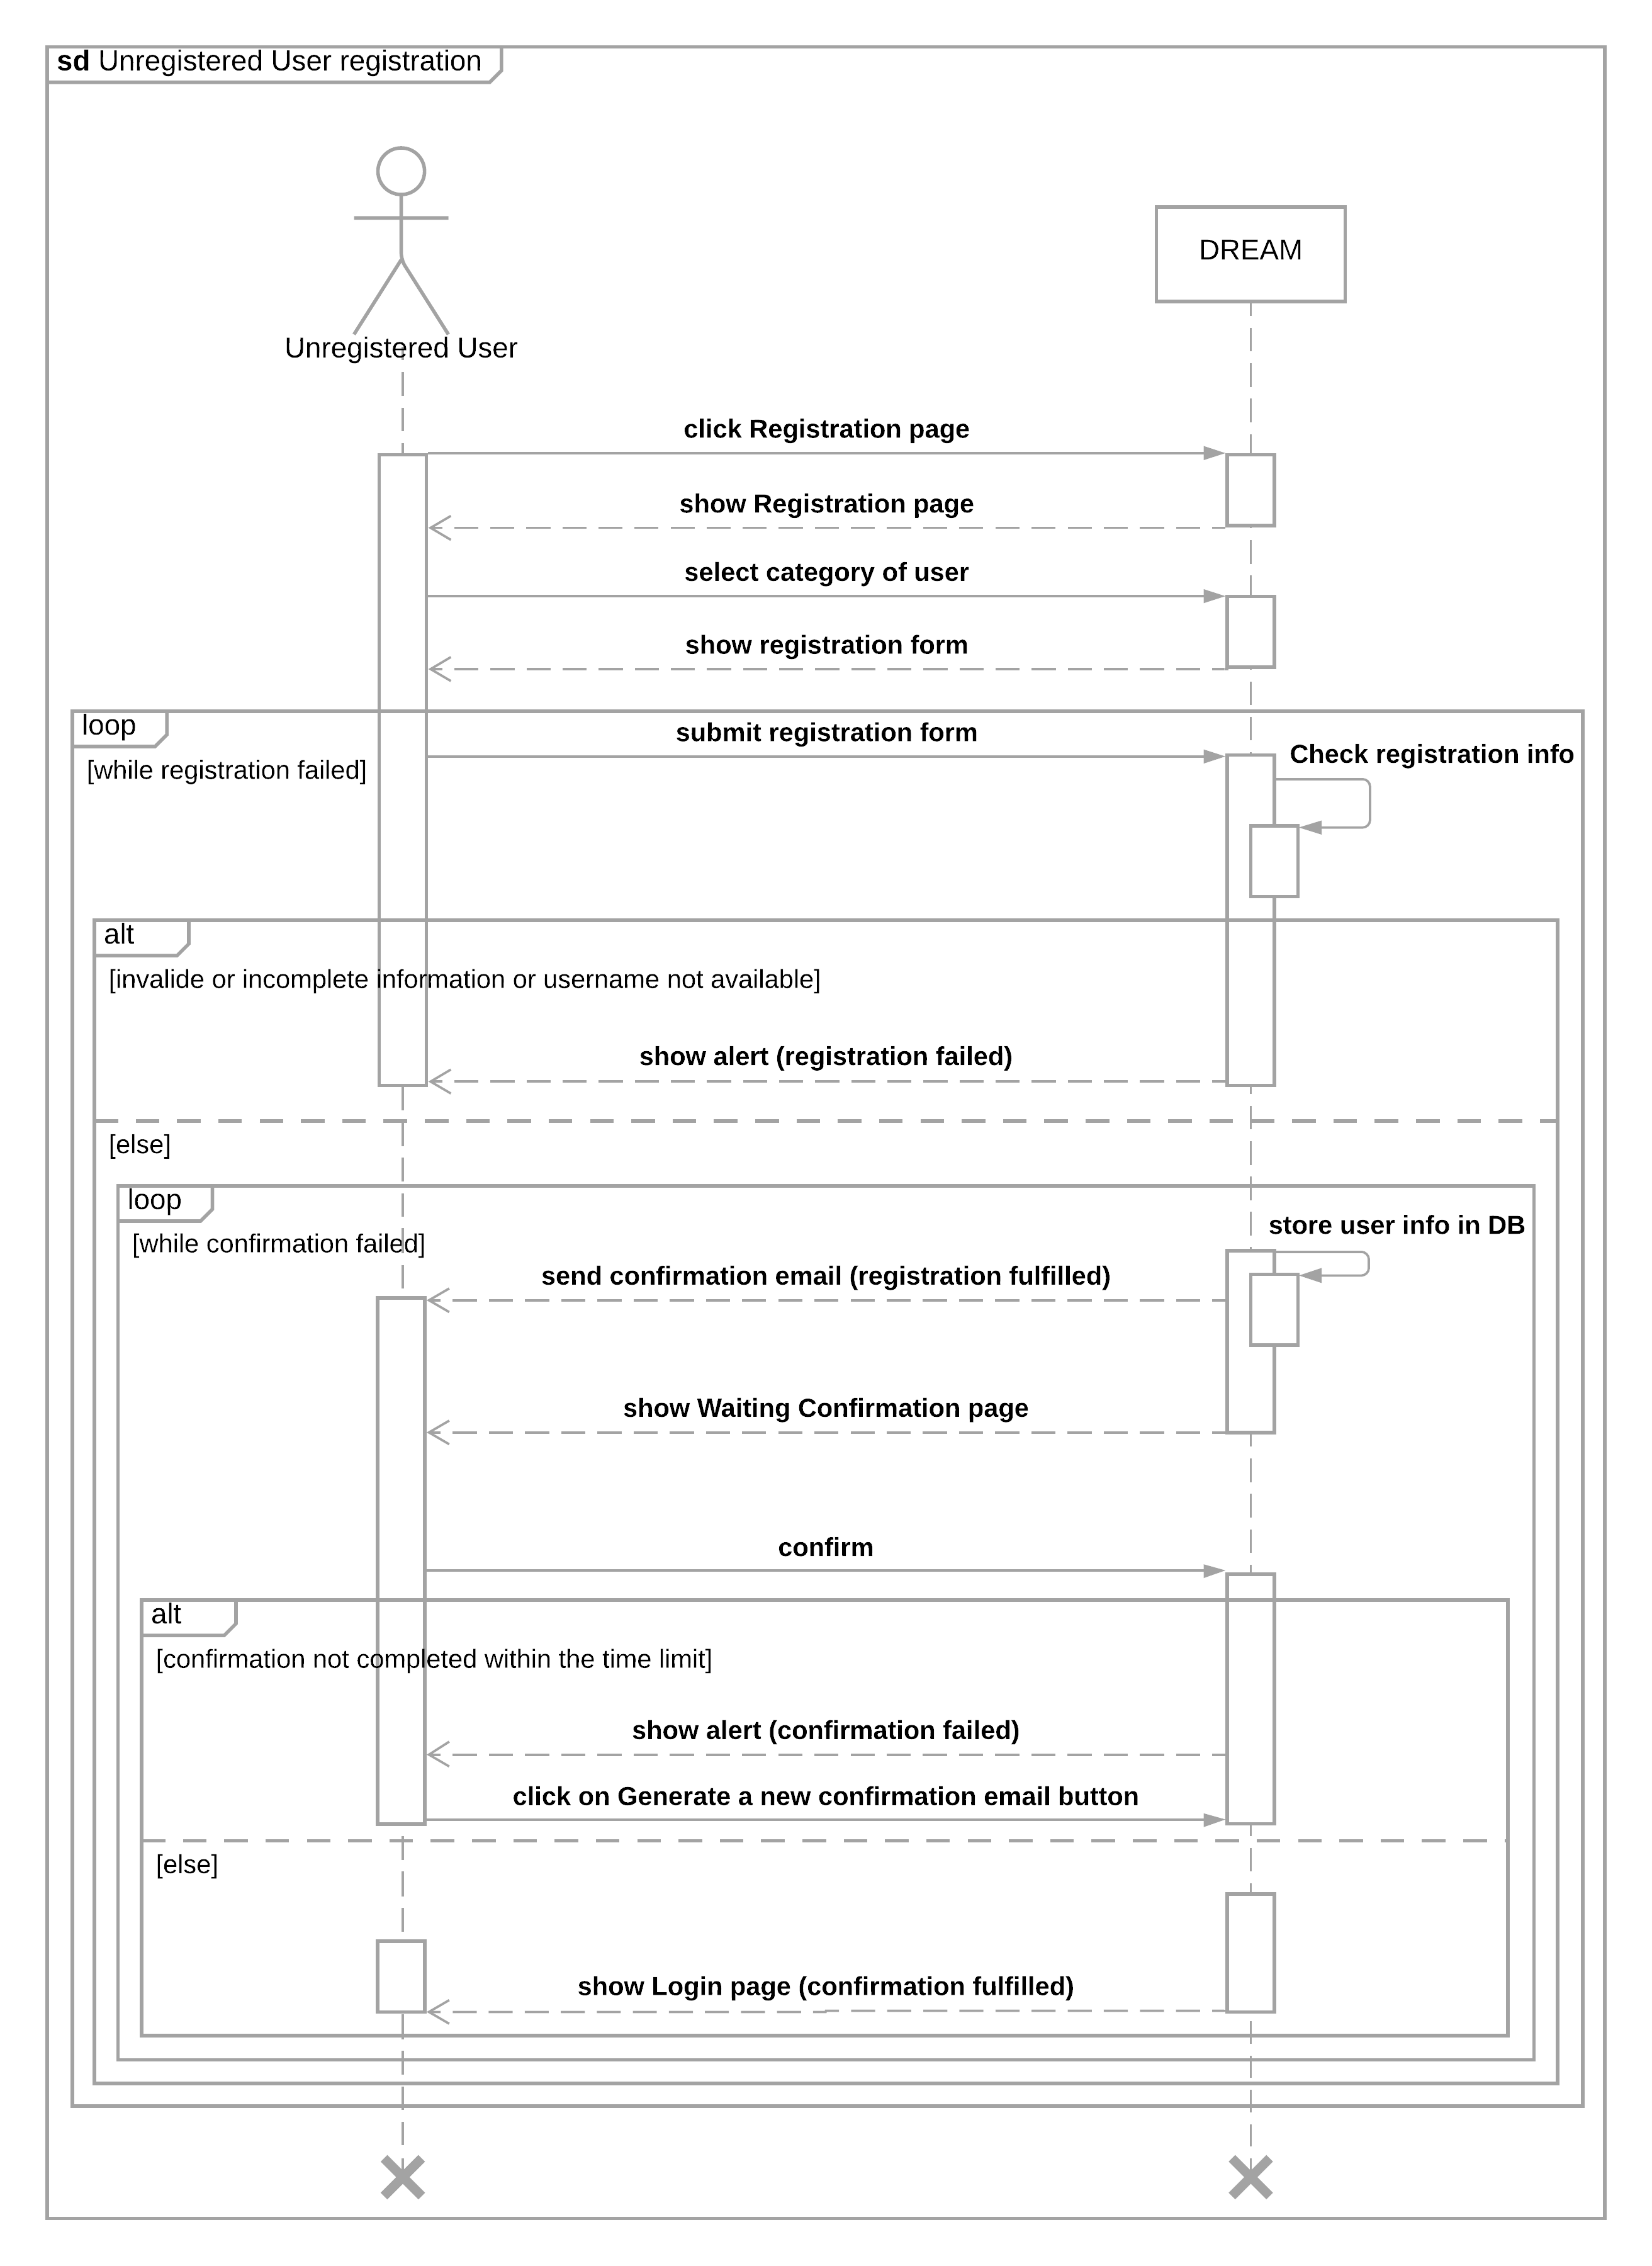
\includegraphics[width=\textwidth,height=\textheight,keepaspectratio]{./Images/Sequence Diagram User Registration.png}
  \caption{Sequence Diagram - Unregistered User Registration}
\end{figure}
\end{center}

\begin{center}
    \begin{figure}[H]
  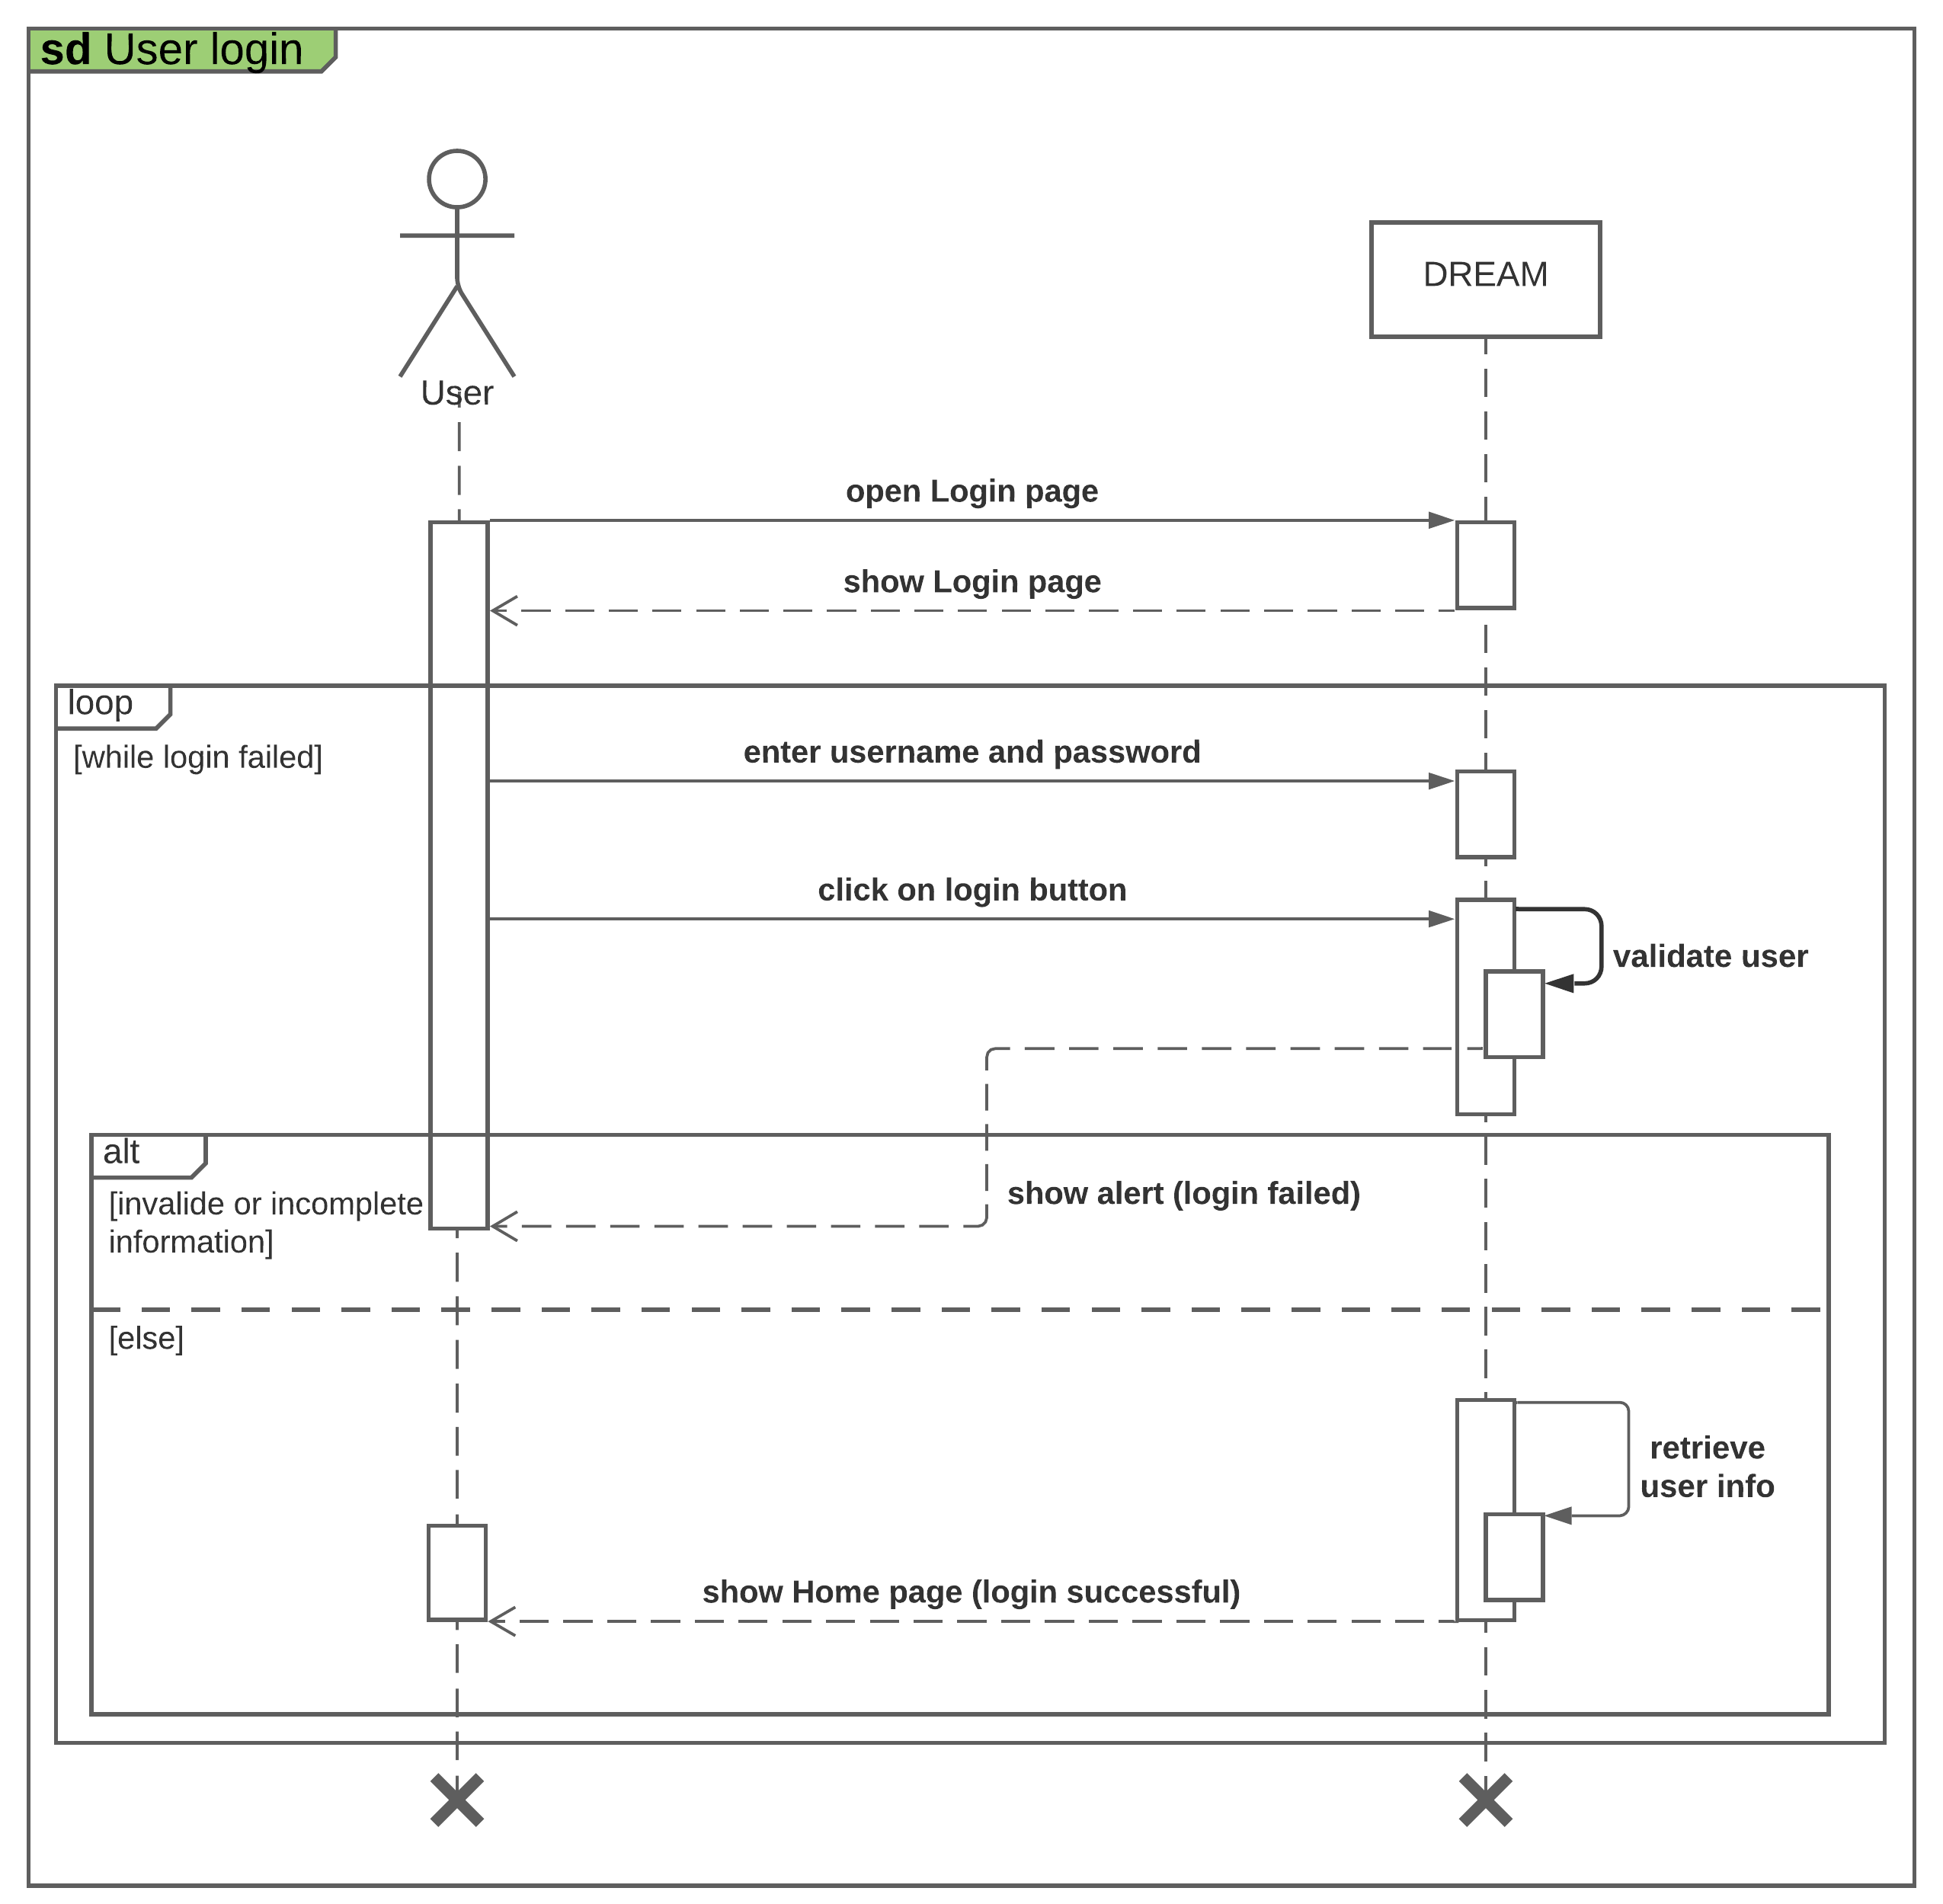
\includegraphics[width=\textwidth,height=\textheight,keepaspectratio]{./Images/Sequence diagram User Login.png}
  \caption{Sequence Diagram - User Login}
\end{figure}

\end{center}
\begin{center}
    \begin{figure}[H]
  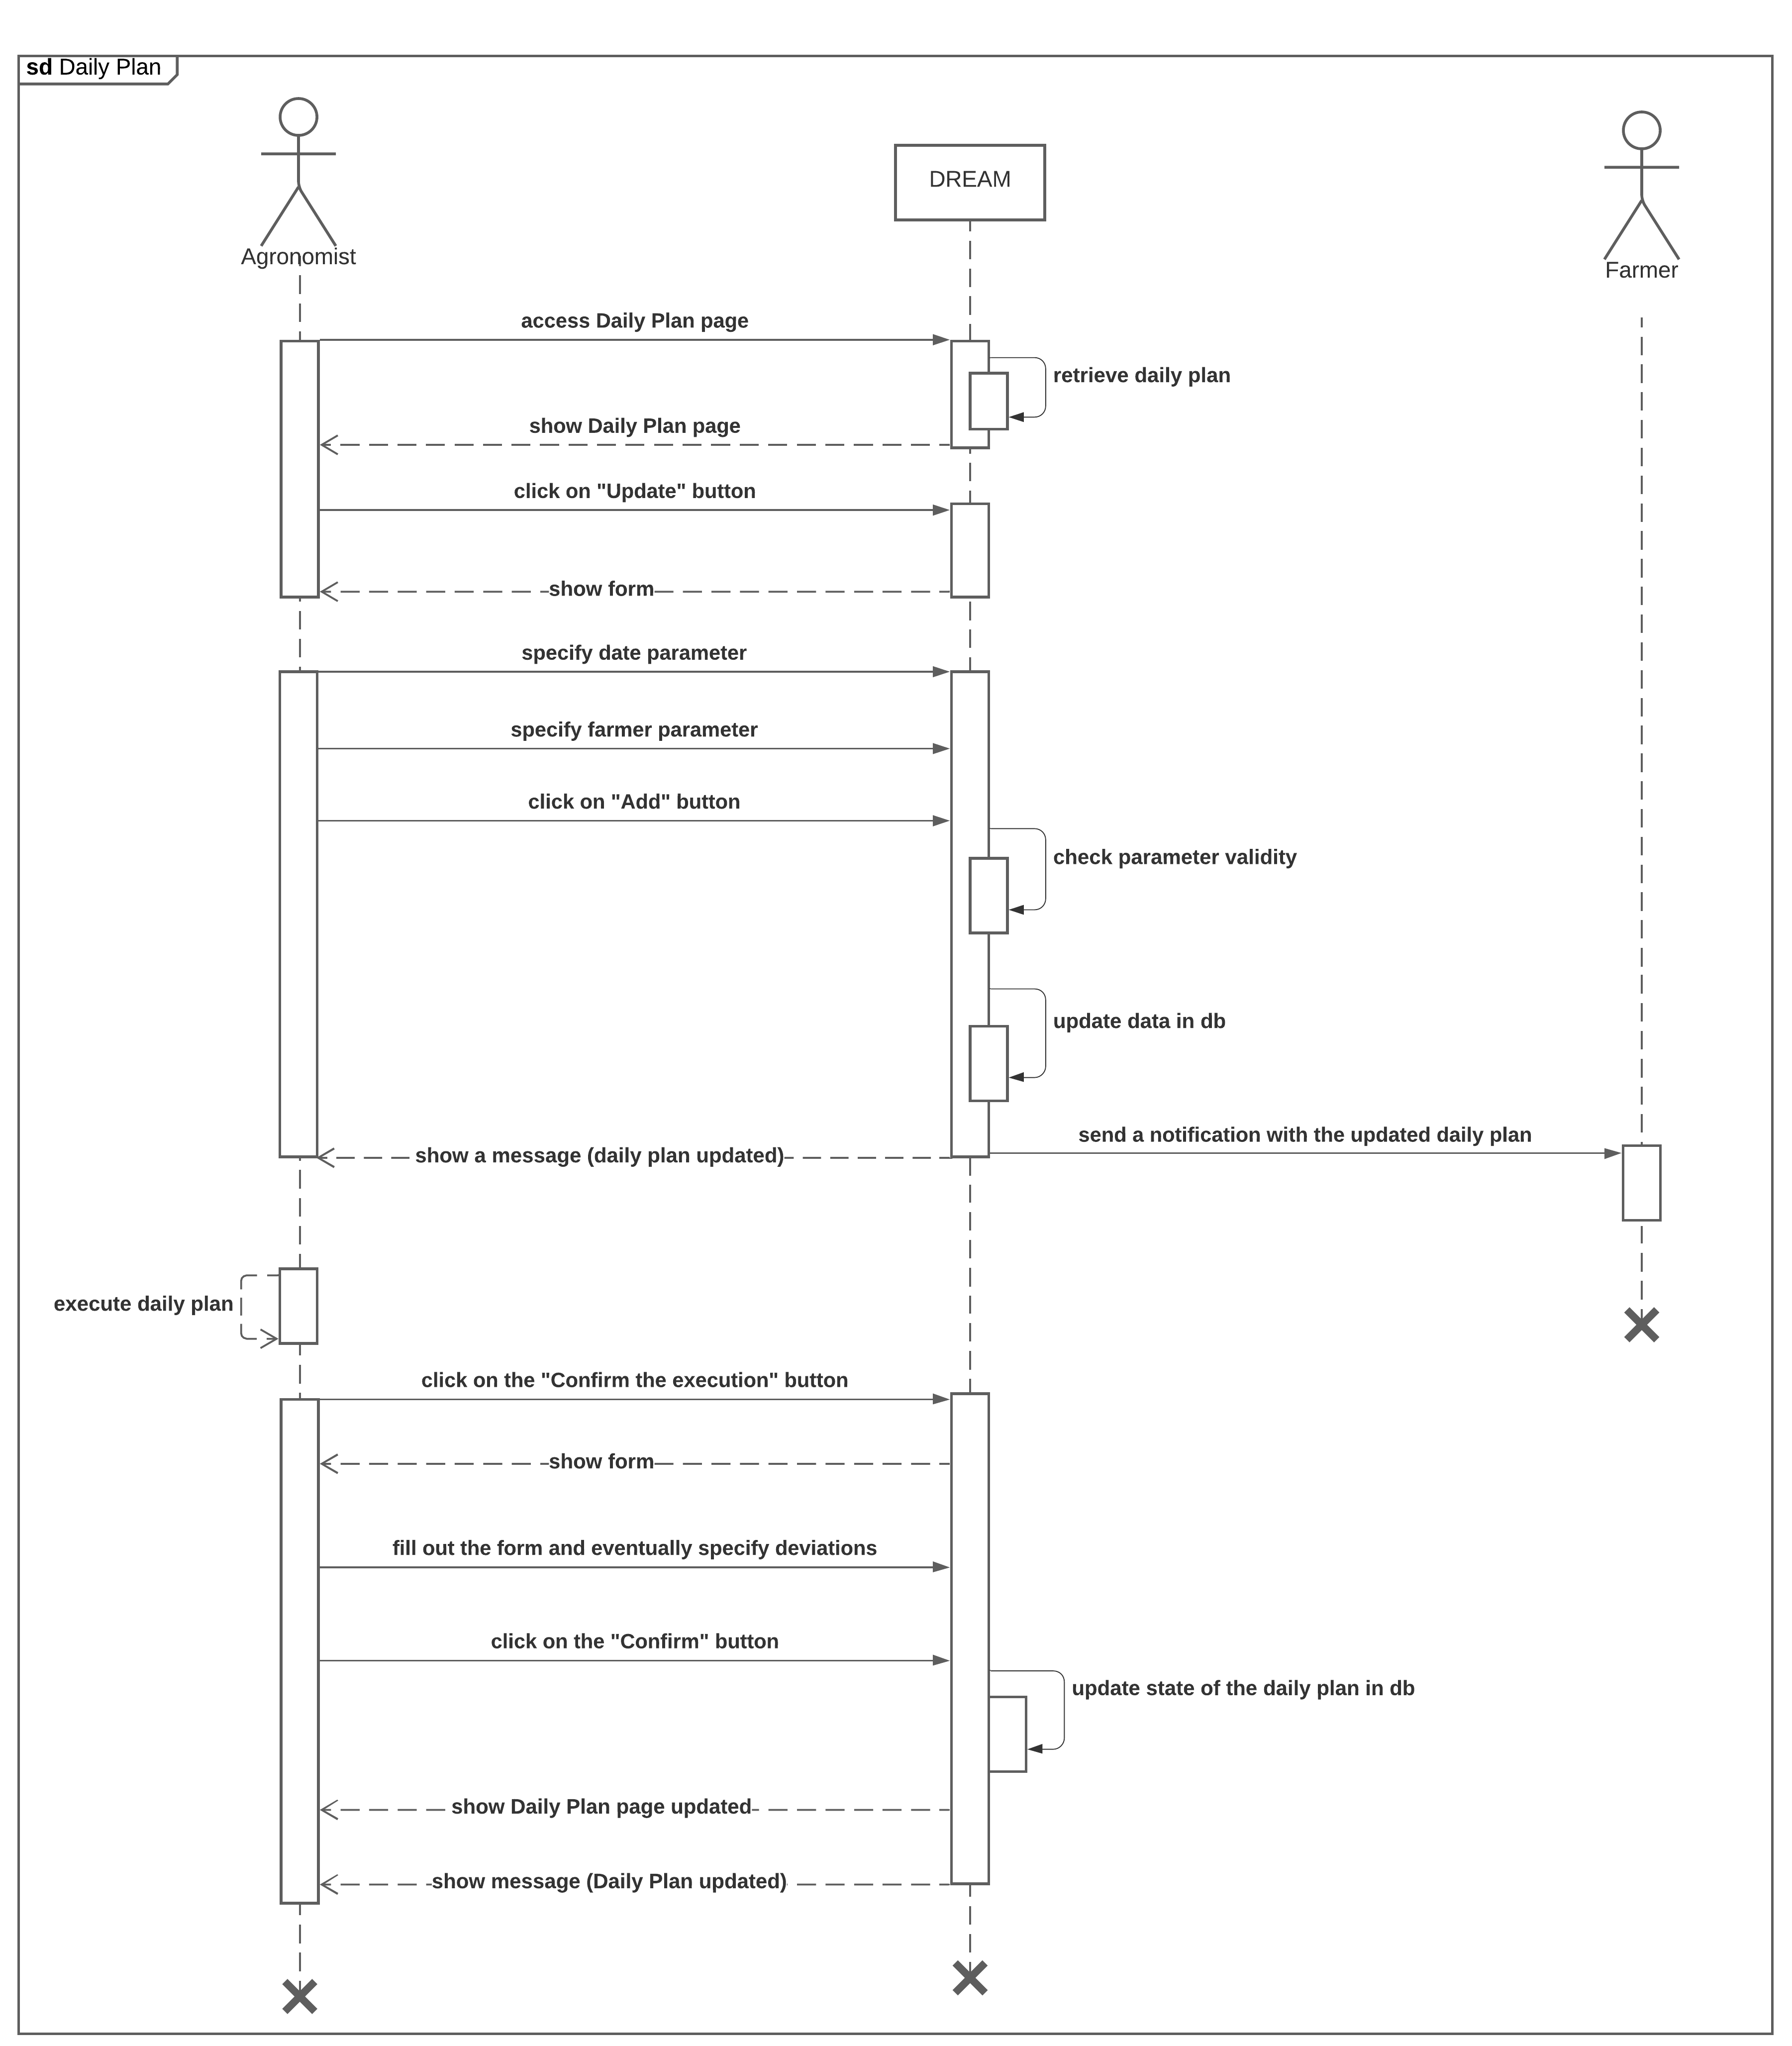
\includegraphics[width=\textwidth,height=\textheight,keepaspectratio]{./Images/Sequence diagram Daily Plan.png}
  \caption{Sequence Diagram - Daily Plan}
\end{figure}
\end{center}

\begin{center}
    \begin{figure}[H]
  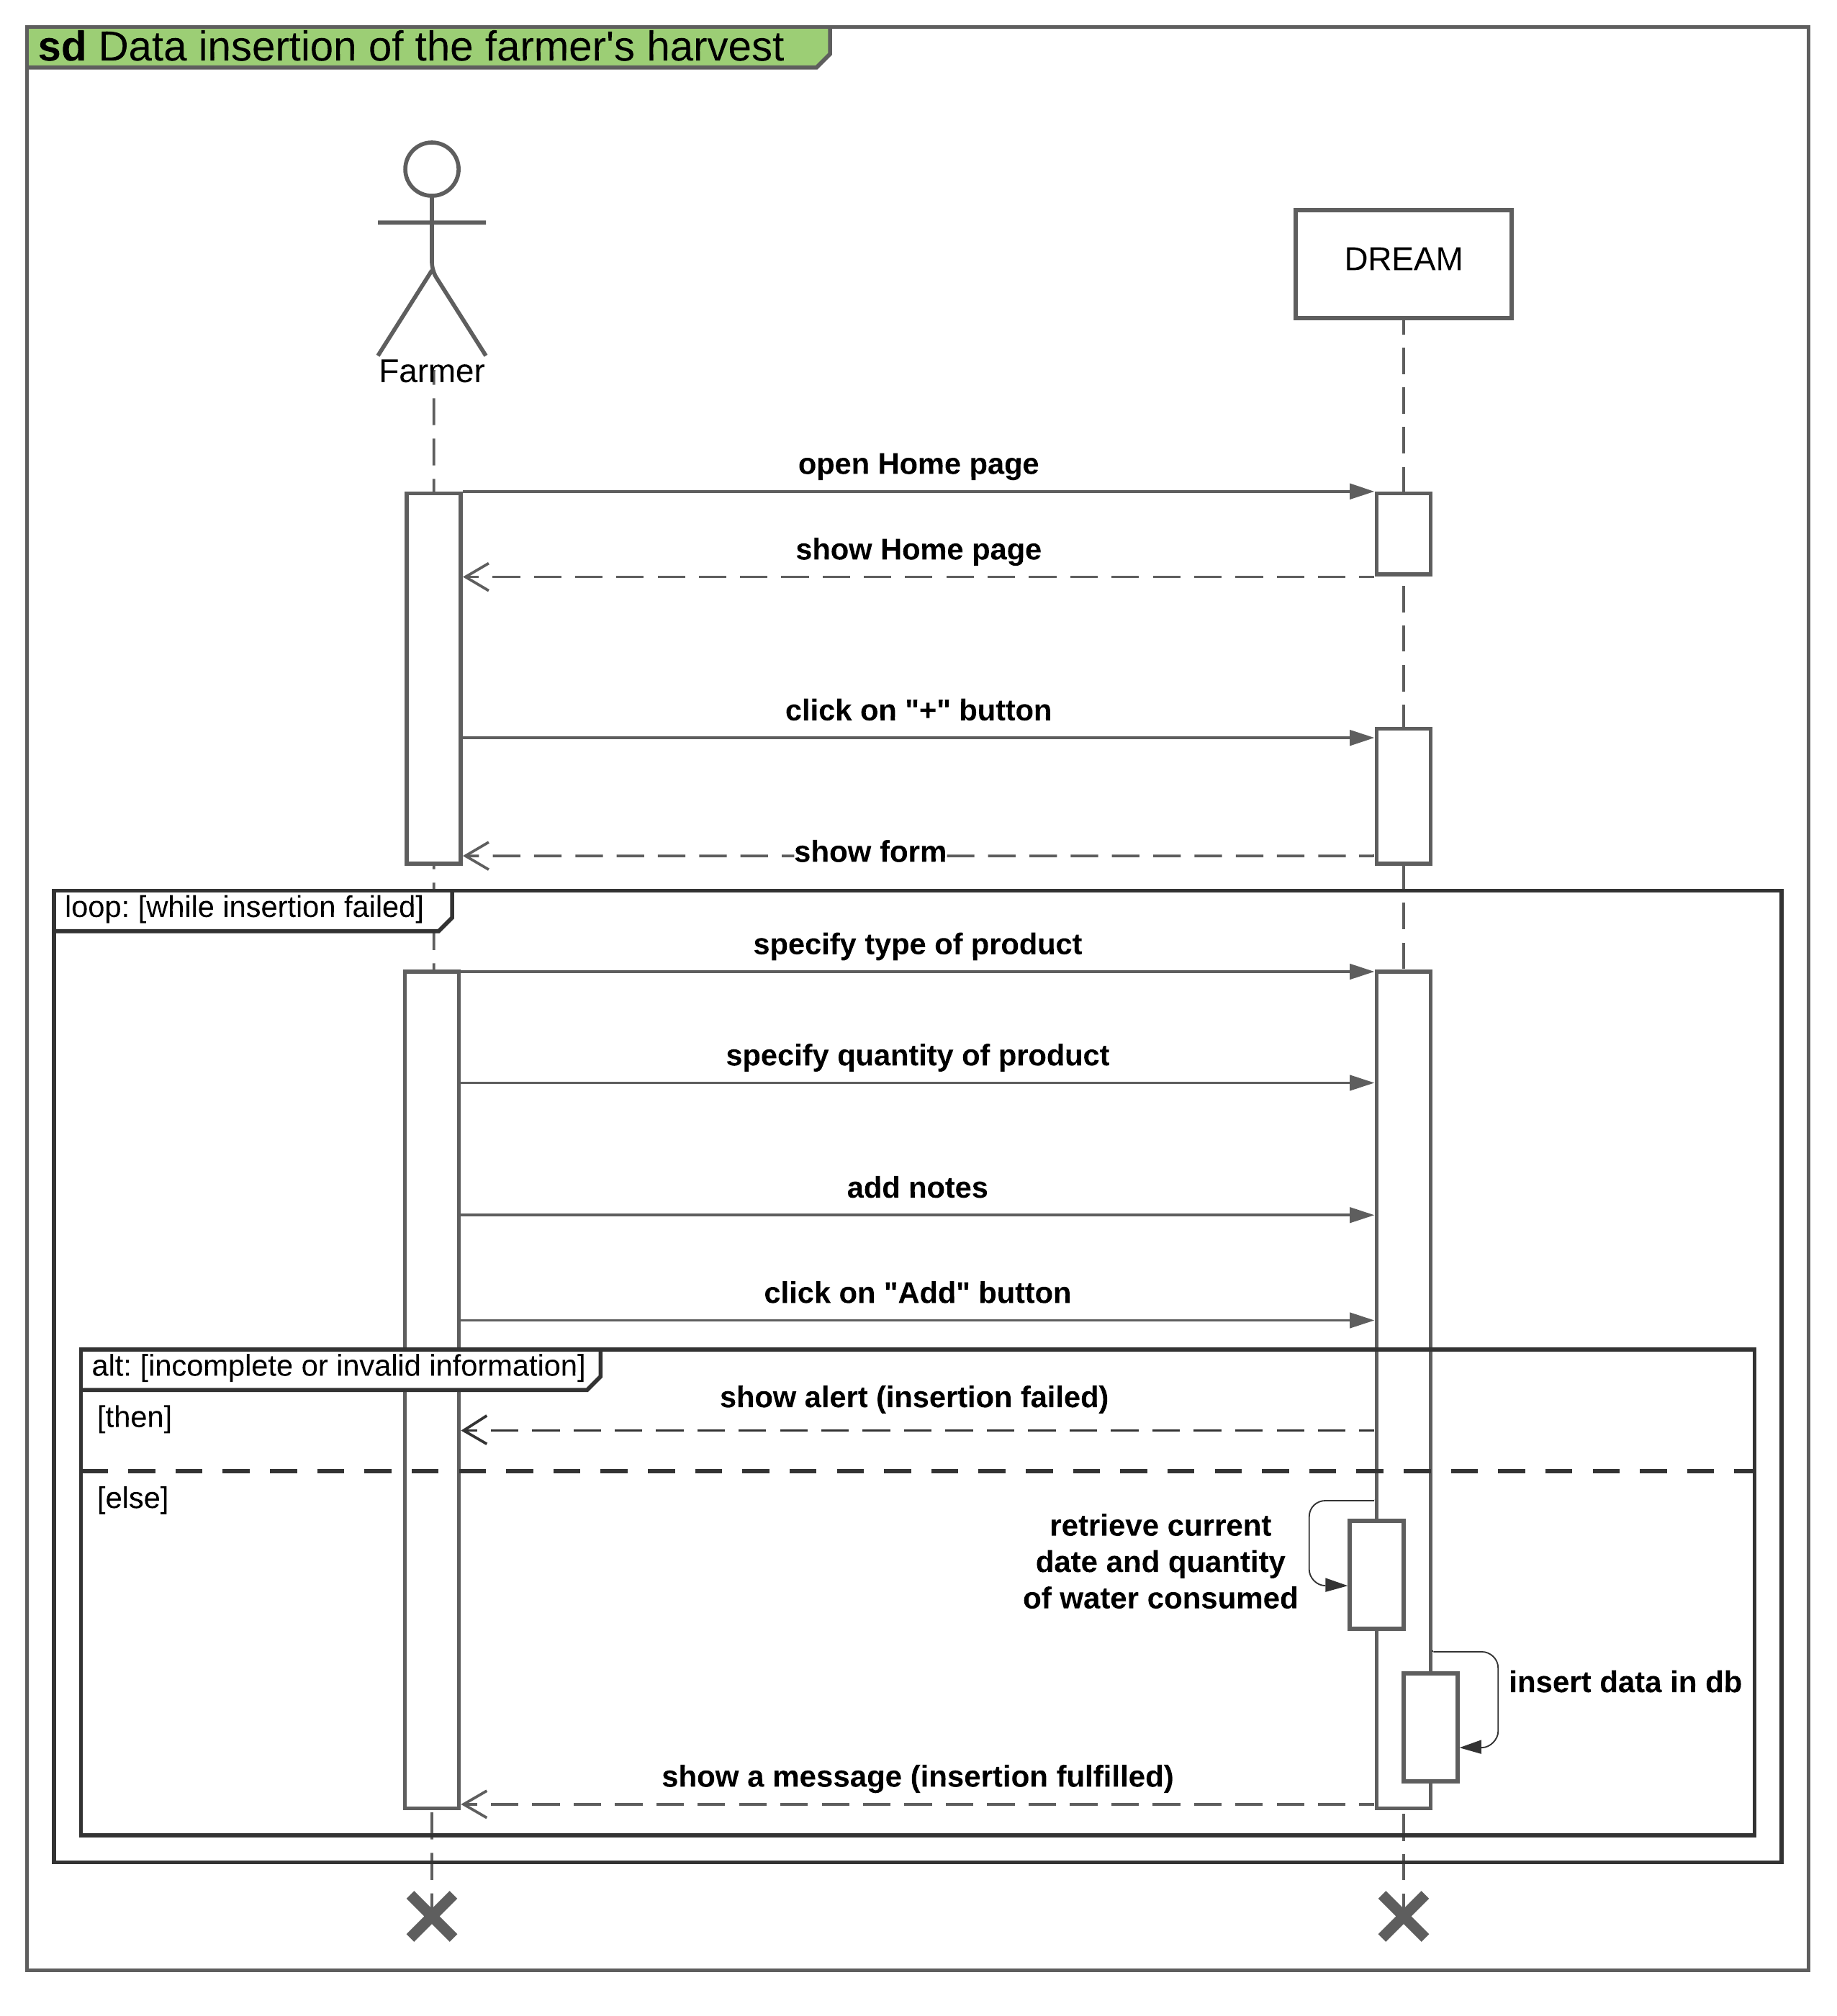
\includegraphics[width=\textwidth,height=\textheight,keepaspectratio]{./Images/Sequence diagram Data insertion of the farmer's harvest.png}
  \caption{Sequence Diagram - Data insertion of the farmer's harvest}
\end{figure}
\end{center}

\begin{center}
    \begin{figure}[H]
  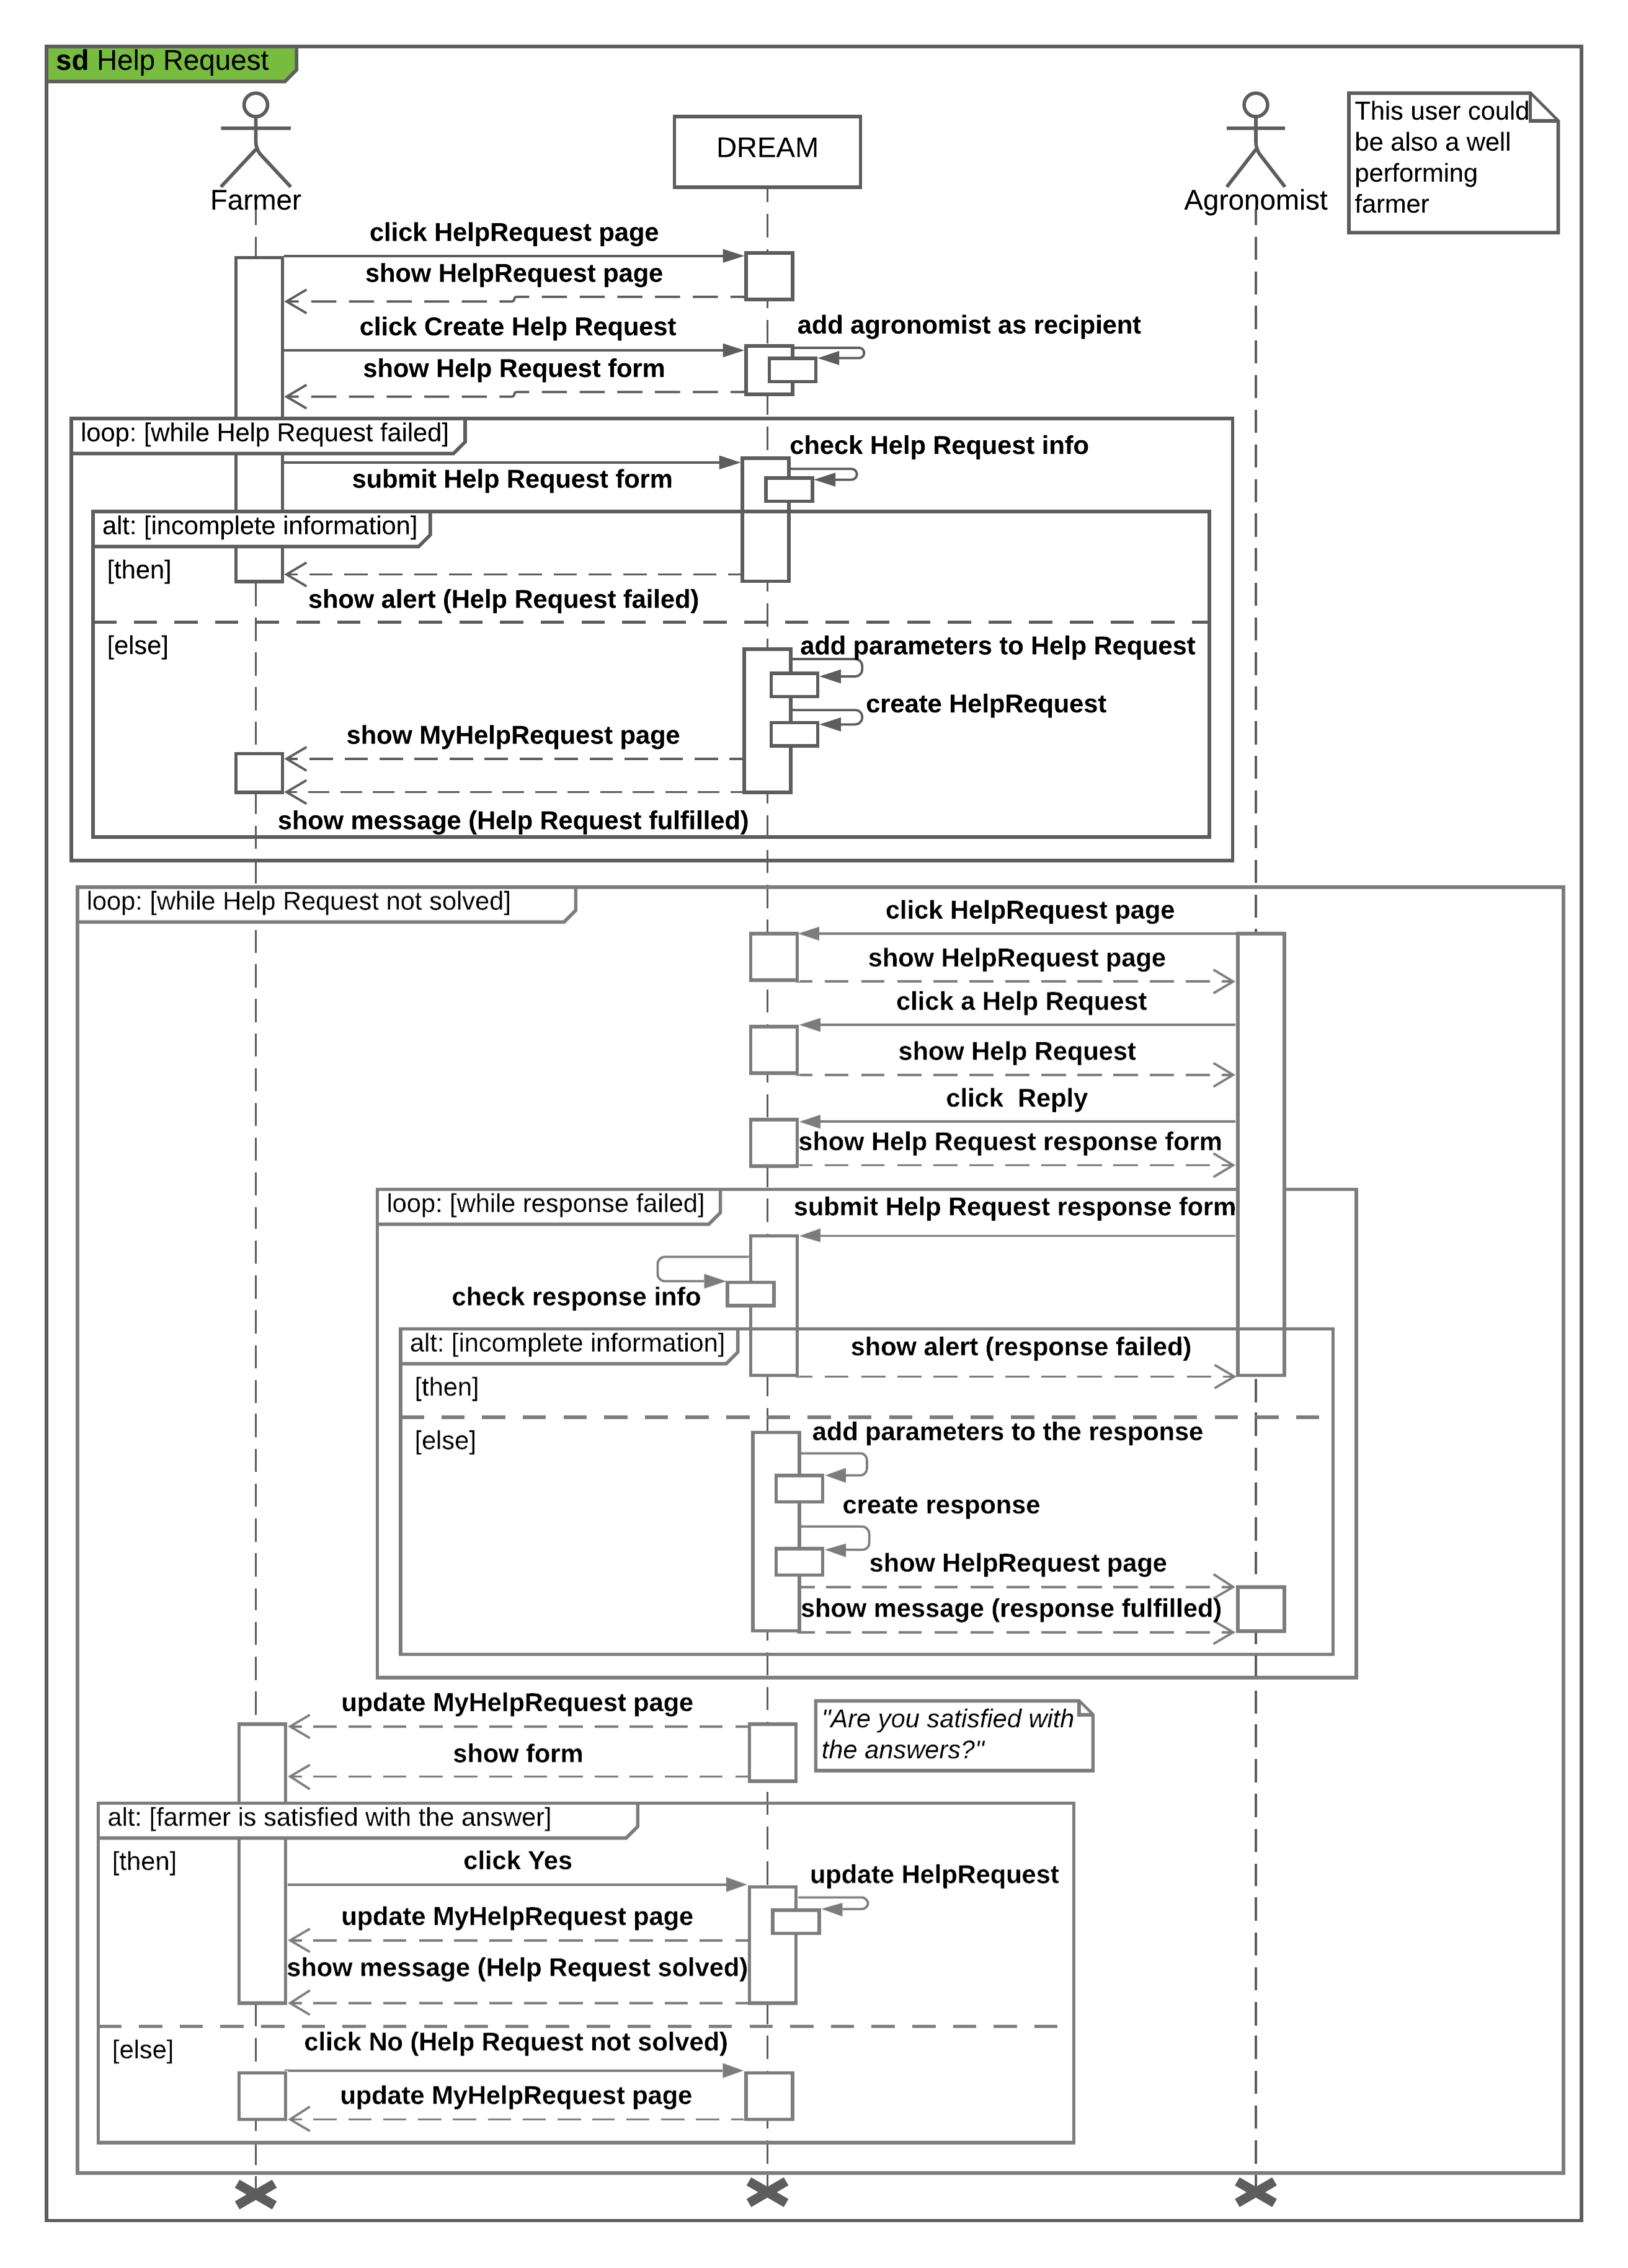
\includegraphics[width=\textwidth,height=\textheight,keepaspectratio]{./Images/Sequence Diagram Help Request.png}
  \caption{Sequence Diagram - Help Request}
\end{figure}
\end{center}




\subsection{Requirements}

In this section are listed all the requirements needed to achieve the goals previously described in \textit{Section 1.1.1}.\\

\textbf{\textcolor{green}{LEGENDA: in verde i requirement che si ripetono più volte}}

\begin{itemize}
     \item [\textit{R.1}] Unregistered User must be able to register to DREAM
    \begin{itemize}
        \item [\textit{R.1.1}] Unregistered User must be able to select his role
        \item [\textit{R.1.2}] Unregistered User must be able to fill out the registration form
    \end{itemize}
    \item [\textit{R.2}] User must be able to login to DREAM by filling out the login form

    \textbf{\item [\textit {G.1}] Allows policy makers to visualize and analyze data of farmers UC17 UC16}
    \item [\textit{R.3}]\textcolor{green}{The system must be able to show the map with performance score regarding farmers}
    \begin{itemize}
    \item [\textit{R.3.1}]\textcolor{green}{The system must be able to identify the farmer's address on the map}
    \item [\textit{R.3.2}]\textcolor{green}{The system must be able to compute performance score of each farmer}
    \item [\textit{R.3.3}] \textcolor{green}{The system must to able to upload most recent computed performance score on the map}
    \item [\textit{R.3.4}] \textcolor{green}{The system must be able to visualize on the map the color associated with each farmer based on his performance score}
    \end{itemize}
    \item [\textit{R.4}]\textcolor{green}{The system must be able to show the farmers information linked to a certain icon in the map}
    \item [\textit{R.5}]The policy maker must be able to select options which he wants to update the map with 
    \begin{itemize}
    \item [\textit{R.5.1}]The policy maker must be able to indicate the mandal he wants to visualize
    \item [\textit{R.5.2}]The policy maker must be able to indicate the data regarding farmers he wants to visualize
    \item [\textit{R.5.3}]The policy maker must be able to indicate the operation he wants to compute data with
    \end{itemize}
    \item [\textit{R.6}]The system must be able to show the updated map according to the option chosen by policy maker.
    \begin{itemize}
    \item [\textit{R.6.1}]The system must be able to compute data according to the chosen operation
    \end{itemize}
    \item [\textit{R.7}]\textcolor{green}{The policy maker must be able to select options for the time chart}
    \begin{itemize}
    \item [\textit{R.7.1}]\textcolor{green}{The policy maker must be able to indicate the mandal he wants to analyze}
    \item [\textit{R.7.2}]\textcolor{green}{The policy maker must be able to indicate the data regarding farmers he wants to analyze}
    \item [\textit{R.7.3}]\textcolor{green}{The policy maker must be able to indicate the operation he wants to compute data with}
    \item [\textit{R.7.4}]\textcolor{green}{The policy maker must be able to indicate the time interval}
    \end{itemize}
    \item [\textit{R.8}]\textcolor{green}{The system must be able to show the time chart according to the option chosen by policy maker.}
    \begin{itemize}
    \item [\textit{R.8.1}]\textcolor{green}{The system must be able to compute data according to the chosen operation}
    \end{itemize}
    
    \textbf{\item [\textit {G.2}] Allows policy makers to identify those farmers who are performing well UC16}
    \item [\textit{R.9}]\textcolor{green}{The system must be able to show the map with performance score regarding farmers}
      \begin{itemize}
    \item [\textit{R.9.1}]\textcolor{green}{The system must be able to identify the farmer's address on the map}
    \item [\textit{R.9.2}]\textcolor{green}{The system must be able to compute performance score of each farmer}
    \item [\textit{R.9.3}] \textcolor{green}{The system must to able to upload most recent computed performance score on the map}
    \item [\textit{R.9.4}] \textcolor{green}{The system must to able to visualize on the map the color associated with each farmer based on his performance score}
    \end{itemize}
    \item [\textit{R.10}]\textcolor{green}{The system must be able to show the farmers information linked to a certain icon in the map}
    
    \textbf{\item [\textit {G.3}] Allows policy makers to identify those farmers who are performing badly UC16}
    \item [\textit{R.11}]\textcolor{green}{The system must be able to show the map with performance score regarding farmers}
    \begin{itemize}
    \item [\textit{R.11.1}]\textcolor{green}{The system must be able to identify the farmer's address on the map}
    \item [\textit{R.11.2}]\textcolor{green}{The system must be able to compute performance score of each farmer}
    \item [\textit{R.11.3}] \textcolor{green}{The system must to able to upload most recent computed performance score on the map}
    \item [\textit{R.11.4}] \textcolor{green}{The system must to able to visualize on the map the color associated with each farmer based on his performance score}
    \end{itemize}
    \item [\textit{R.12}]\textcolor{green}{The system must be able to show the farmers information linked to a certain icon in the map}
    
    \textbf{\item [\textit {G.4}] Allows policy makers to verify the improvement of farmers who have been already helped by agronomist or good farmers UC17}
    \item [\textit{R.13}]\textcolor{green}{The policy maker must be able to select options for the time chart}
    \begin{itemize}
    \item [\textit{R.13.1}]\textcolor{green}{The policy maker must be able to indicate the mandal he wants to analyze}
    \item [\textit{R.13.2}]\textcolor{green}{The policy maker must be able to indicate the data regarding farmers he wants to analyze}
    \item [\textit{R.13.3}]\textcolor{green}{The policy maker must be able to indicate the operation he wants to compute data with}
    \item [\textit{R.13.4}]\textcolor{green}{The policy maker must be able to indicate the time interval}
    \item [\textit{R.13.5}]The policy maker must be able to visualize data about farmers with help request solved
    \end{itemize}
    \item [\textit{R.14}]\textcolor{green}{The system must be able to show the time chart according to the option chosen by policy maker.}
    \begin{itemize}
    \item [\textit{R.14.1}]\textcolor{green}{The system must be able to compute data according to the chosen operation}
    \end{itemize}
    

     \textbf{\item [\textit {G.5}] Allows farmers to visualize data and suggestions relevant to them based on their location and type of production} UC20 (data) UC14 (comprende suggestions)
    
    \textcolor{red}{Di seguito c'è goal farmer visualize relevant information}
    \item [\textit{R.15}] The system must be able to show weather conditions and soil moisture regarding farmer’s position and the next visit scheduled by the associated agronomist
    \item [\textit{R.15}] The farmer must be able to visualize all visits scheduled for him
    \begin{itemize}
    \item [\textit{R.15.1}] The system must be able to show all scheduled visits in chronological order (even ones that have already occurred in the past)
    \end{itemize}
    
     \textcolor{red}{Di seguito c'è goal farmer receives notifications}
    \item [\textit{R.16}]The system must be able to send notifications to the farmer 
    \begin{itemize}
        \item [\textit{R.16.1}] The system must be able to send notification to the farmer regarding personalized suggestions
        \begin{itemize}
            \item [\textit{R.16.1.1}] The system must be able to compute suggestions according to the information inserted by the farmer and his position
        \end{itemize}
        \item [\textit{R.16.2}] The system must be able to send notification to the farmer regarding new visits scheduled in the daily plan regarding him/her
        \item [\textit{R.16.3}] The system must be able to send notification to the farmer regarding new answers to his created Help Requests not yet solved 
        \item [\textit{R.16.4}] The system must be able to send notification to the farmer regarding new answers to his threads on the Discussion Forum
    \end{itemize}
    \item [\textit{R.17}] The farmer must be able to visualize notifications' details
    \item [\textit{R.18}] The system must be able to show the details regarding the notification selected by the farmer
    \item [\textit{R.19}] The system must be able to show a list of the notifications received in chronological order
    
    
    \textbf{\item [\textit {G.6}] Allows farmers to insert in the system data about their production and any problem they face} UC3
    \item [\textit{R.20}] Farmer must be able to fill out the form for data insertion
    \begin{itemize}
    \item [\textit{R.20.1}] Farmer must be able to insert the type of product of his harvest
    \item [\textit{R.20.2}] Farmer must be able to insert the quantity of product of his harvest
    \item [\textit{R.20.3}] Farmer must be able to insert note about his harvest
    \item [\textit{R.20.4}] \textcolor{green}{The system must be able to return a message in case of successful data insertion} 
    \item [\textit{R.20.5}] \textcolor{green}{The system must be able to return an alert in case of failed data insertion}
    \end{itemize}
    \item [\textit{R.21}] The system must be able to add parameters to the inserted data
    \begin{itemize}
    \item [\textit{R.21.1}] The system must be able to add the current date to the inserted data
    \item [\textit{R.21.2}] The system must be able to add the quantity of water consumed to the inserted data
    \end{itemize}
    
    \textbf{\item [\textit {G.7}] Allows farmers to request for help and suggestions by agronomists and other farmers} UC4
    \item [\textit{R.22}]The farmer must be able to request for help by filling a form
    \begin{itemize}
    \item [\textit{R.22.1}]The system must be able to add agronomist as recipient of the Help Request by default
    \item [\textit{R.22.2}]The farmer must be able whether to select well performing farmer as recipients of the Help Request or not
    \item [\textit{R.22.3}] The farmer must be able to write the body of the Help Request in the appropriate field
    \item [\textit{R.22.4}] \textcolor{green}{The system must be able to return a message in case of successful data insertion}
    \item [\textit{R.22.5}] \textcolor{green}{The system must be able to return an alert in case of failed data insertion}
    \end{itemize}
    \item [\textit{R.23}] The system must be able to add parameters to the Help Request
    \begin{itemize}
    \item [\textit{R.23.1}] The system must be able to add the username of the farmer to the Help Request
    \item [\textit{R.23.2}] The system must be able to add the current date to the help request
    \item [\textit{R.23.2}] The system must be able to add the status created to the Help Request
    \end{itemize}
    
\textcolor{red}{qui di seguito c'è a farmer solves a help request UC5}
 \item [\textit{R.24}]The farmer must be able to solve a Help Request
    \begin{itemize}
    \item [\textit{R.24.1}] The system must be able to show the list of all the help requests of the farmer created, but not solved
    \item [\textit{R.24.2}]The system must be able to show a message regarding the level of satisfaction of the farmer when a Help Request is replied
    \item [\textit{R.24.3}] The farmer must be able to select an answer 
    \item [\textit{R.24.4}] The system must be able to change the status of the Help Request into solved in the DB
    \item [\textit{R.24.5}] The system must be able to return a message in case of Help Request solved
    \end{itemize}

    
    
    \textbf{\item [\textit {G.8}] Allows farmers to create discussion forums with the other farmers} UC6 UC7 UC8
    
    \item [\textit{R.25}] The system must be able to show a list of existing threads only visualizing the associated topic
    \item [\textit{R.26}] The farmer must be able to visualize a certain thread with related answers
        \begin{itemize}
            \item [\textit{R.26.1}] The farmer must be able to select an already existing thread
            \item [\textit{R.26.2}] The system must be able to show the selected thread with all associated answers
    \end{itemize}
      
    \textcolor{red}{Di seguito c'è farmer searches for a topic}
      
    \item [\textit{R.27}]The farmer must be able to search for a topic on the discussion forum
    \begin{itemize}
        \item [\textit{R.27.1}] The farmer must be able to fill out a form to search for a topic in the forum
        \begin{itemize}
        \item [\textit{R.27.1.1}]The farmer must be able to insert in the form the topic to be searched
        \item [\textit{R.27.1.2}] \textcolor{green}{The system must be able to return a message in case of successful data insertion}
        \item [\textit{R.27.1.3}] \textcolor{green}{The system must be able to return an alert in case of failed data insertion}
        \end{itemize}
    \item [\textit{R.27.2}]The system must be able to show a list of already existing threads associated to the searched topic
    \item [\textit{R.27.3}]The system must be able to show a message in case of no existing threads associated to the searched topic, to suggest to attempt a new research or to open a new thread
    \end{itemize}
    
    \textcolor{red}{Di seguito c'è farmer opens a thread}
    
    \item [\textit{R.28}]The farmer must be able to open a thread on the discussion forum
    \begin{itemize}
        \item [\textit{R.28.1}] The farmer must be able to fill out a form to open a thread on the discussion forum
        \begin{itemize}
        \item [\textit{R.28.1.1}]The farmer must be able to insert in the form the topic of the thread
        \item [\textit{R.28.1.2}] The farmer must be able to insert in the form the text of the thread
        \item [\textit{R.28.1.3}] \textcolor{green}{The system must be able to return a message in case of successful data insertion}
        \item [\textit{R.28.1.4}] \textcolor{green}{The system must be able to return an alert in case of failed data insertion}
        \end{itemize}
        \item [\textit{R.28.2}] The system must be able to add parameters to the thread
    \begin{itemize}
    \item [\textit{R.28.2.1}] The system must be able to add the username of the farmer to the thread
    \item [\textit{R.28.2.2}] The system must be able to add the current date to the thread
    \end{itemize}
    \end{itemize}
    
    \textcolor{red}{Di seguito c'è farmer answers to a thread}
    
    \item [\textit{R.29}]The farmer must be able to answer on the discussion forum
        \begin{itemize}
        \item [\textit{R.29.1}] The farmer must be able to fill out a form to reply to a thread
        \begin{itemize}
        \item [\textit{R.29.1.1}]The farmer must be able to insert in the form the text of the response
        \item [\textit{R.29.1.2}] \textcolor{green}{The system must be able to return a message in case of successful data insertion}
        \item [\textit{R.29.1.3}] \textcolor{green}{The system must be able to return an alert in case of failed data insertion}
        \end{itemize}
        \item [\textit{R.29.2}] The system must be able to add parameters to the response
    \begin{itemize}
    \item [\textit{R.29.2.1}] The system must be able to add the username of the farmer to the response
    \item [\textit{R.29.2.2}] The system must be able to add the current date to the response
    \end{itemize}
    \end{itemize}
    
    
    \textbf{\item [\textit {G.9}] Allows agronomists to receive information about requests for help} UC11
    \item [\textit{R.30}]The system must be able to notify the agronomist when a new Help Request is created and not yet solved
    \item [\textit{R.31}] The agronomist must be able to visualize notification's details
    \item [\textit{R.32}] The system must be able to show the details regarding the notification selected by the agronomist
    \item [\textit{R.33}] The system must be able to show a list of the notifications received in chronological order
    
    
    
    \textbf{\item [\textit {G.10}] Allows agronomists to answer to requests for help from farmers} UC12
    \item [\textit{R.34}]The agronomist must be able to answer to a Help Request
    \item [\textit{R.35}] The system must be able to show a list of the Help Requests created and not yet solved. 
    \item [\textit{R.36}] The agronomist must be able to select a Help Request to read its details
    \item [\textit{R.37}] The system must be able to show the details of the Help Request selected by the agronomist
    \begin{itemize}
        \item [\textit{R.37.1}] The agronomist must be able to fill out a form to reply to the Help Request
        \begin{itemize}
        \item [\textit{R.37.2}]The agronomist must be able to insert in the form the text of the response
        \item [\textit{R.37.3}] \textcolor{green}{The system must be able to return a message in case of successful data insertion}
        \item [\textit{R.37.4}] \textcolor{green}{The system must be able to return an alert in case of failed data insertion}
        \end{itemize}
        \item [\textit{R.37.5}] The system must be able to add parameters to the response
            \begin{itemize}
                \item [\textit{R.37.5.1}] The system must be able to add the full name of the agronomist to the response
                \item [\textit{R.37.5.2}] The system must be able to add the current date to the response
    \end{itemize}
    \end{itemize}
    
 \textcolor{red}{\textbf{\item Allows well performing farmers to answer to requests for help from farmers} UC13}
    \item [\textit{R.38}]The system must be able to compute performance score of each farmer
    \item [\textit{R.39}]The system must be able to classify farmers according to their performance score value 
    \item [\textit{R.40}]The well performing farmer must be able to answer to a Help Request
    \item [\textit{R.41}] The system must be able to show a list of the Help Requests created and not yet solved with well performing farmers as recipient. 
    \item [\textit{R.42}] The well performing farmer must be able to select a Help Request to read its details
    \item [\textit{R.43}] The system must be able to show the details of the Help Request selected by the well performing farmers
    \begin{itemize}
        \item [\textit{R.43.1}] The well performing farmer must be able to fill out a form to reply to the Help Request
        \begin{itemize}
        \item [\textit{R.43.2}]The well performing farmer must be able to insert in the form the text of the response
        \item [\textit{R.43.3}] \textcolor{green}{The system must be able to return a message in case of successful data insertion}
        \item [\textit{R.43.4}] \textcolor{green}{The system must be able to return an alert in case of failed data insertion}
        \end{itemize}
        \item [\textit{R.43.5}] The system must be able to add parameters to the response
            \begin{itemize}
                \item [\textit{R.43.5.1}] The system must be able to add the username of the well performing farmer to the response
                \item [\textit{R.43.5.2}] The system must be able to add the current date to the response
    \end{itemize}
    \end{itemize}
    

    \textbf{\item [\textit {G.11}] Allows agronomists to visualize data concerning farmers in the mandal} UC15
    \item [\textit{R.44}]\textcolor{green}{The system must be able to show the map with performance score regarding farmers of his mandal}
    \begin{itemize}
    \item [\textit{R.44.1}]\textcolor{green}{The system must be able to identify the farmer's address on the map}
    \item [\textit{R.44.2}]\textcolor{green}{The system must be able to compute performance score of each farmer}
    \item [\textit{R.44.3}] \textcolor{green}{The system must to able to upload most recent computed performance score on the map}
    \item [\textit{R.44.4}] \textcolor{green}{The system must to able to visualize on the map the color associated with each farmer based on his performance score}
    \end{itemize}
    \item [\textit{R.45}]\textcolor{green}{The system must be able to show the farmers information linked to a certain icon in the map}
    \item [\textit{R.46}]The system must be able to show a table with best performing farmers data
    
    
    \textbf{\item [\textit {G.12}] Allows agronomists to visualize weather forecasts in the mandal} UC19
    \item [\textit{R.47}]The system must be able to show the map of his mandal with weather conditions and soil moisture of the current date
    \item [\textit{R.48}]The agronomist must be able to visualize weather forecasts up to seven day after the current date
    \begin{itemize}
        \item [\textit{R.48.1}]The agronomist must be able to select the day  for which he wants to visualize weather forecasts
        \item [\textit{R.48.2}] \textcolor{green}{The system must be able to return a message in case of successful data insertion}
        \item [\textit{R.48.3}] \textcolor{green}{The system must be able to return an alert in case of failed data insertion}
        \item [\textit{R.48.4}]The system must be able to show the updated mandal map with weather forecasts regarding the day selected by the agronomist
    \end{itemize}
    
    
    
    \textbf{\item [\textit {G.13}] Allows agronomists to visualize a daily plan to visit farms in the mandal} UC18
    \item [\textit{R.49}] The system must be able to show the Daily Plan of the current day
    \begin{itemize}
        \item [\textit{R.49.1}]The system must be able to compute the Daily Plan assigning two visits per year to each farmer
        \item The system must be able to set the status of the daily plan into created in the DB 
    \end{itemize}
    
    \textbf{\item [\textit {G.14}] Allows agronomists to update a daily plan to visit farms in the mandal} UC9
    
    \textbf{\item [\textit {G.15}] Allows agronomists to confirm the execution of the daily plan at the end of each day} UC10
    
    \textbf{\item [\textit {G.16}] Allows agronomists to specify the deviations from the daily plan at the end of the day} UC10
    
    \textcolor{red}{Di seguito c'è agronomist updates daily plan} 
    \item [\textit{R.50}]The agronomist must be able to update the Daily Plan
    \begin{itemize}
        \item [\textit{R.50.1}] The agronomist must be able to fill out a form to update the Daily Plan
        \begin{itemize}
        \item [\textit{R.50.1.1}] The agronomist must be able to insert in the form the date of the day he wants to update in the Daily Plan
        \item [\textit{R.50.1.2}] The agronomist must be able to insert in the form the farmer related to the visit which the agronomist is updating the Daily Plan with
        \item [\textit{R.50.1.3}] \textcolor{green}{The system must be able to return a message in case of successful data insertion}
        \item [\textit{R.50.1.4}] \textcolor{green}{The system must be able to return an alert in case of failed data insertion}
        \end{itemize}
        \item [\textit{R.50.2}] The system must be able to add parameters to the updating visit 
    \begin{itemize}
    \item [\textit{R.50.2.1}] The system must be able to add the full name of the agronomist to the updating visit
    \end{itemize}
    \end{itemize}
    \item [\textit{R.51}]The system must be able to change the status of the daily plan into updated in the DB
    
    \textcolor{red}{Di seguito c'è agronomist confirms daily plan} 
        
    \item [\textit{R.52}]The agronomist must be able to confirm the Daily Plan
    \begin{itemize}
        \item [\textit{R.52.1}] The agronomist must be able to fill out a form to confirm the Daily Plan
        \begin{itemize}
        \item [\textit{R.52.1.1}] The agronomist must be able to insert in the form deviations from the plan
        \end{itemize}
    \end{itemize}
    \item [\textit{R.53}]The system must be able to change the status of the daily plan into done in the DB
\end{itemize}
\subsection{Traceability Matrix}

In this section is reported a detailed mapping between requirements defined in \textit{Subsection 3.2.4} and goals of the application listed in \textit{Subsection 1.1.1}, which are achieved under the domain assumptions defined in \textit{Subsection 2.4.1}.


\rowcolors{2}{white}{white!65!green2!50}
\setlength\tabcolsep{5pt}
\renewcommand{\arraystretch}{1.7}
\begin{longtable}{|m{0.9cm}|m{5.2cm}|m{5.2cm}|}
\caption{Traceability Matrix\label{long}}\\
\hline
\endfirsthead
\endhead
\hline
\endlastfoot
\rowcolor{green2}
\textbf{Goal} & \hfil{\textbf{Domain Assumptions}} & \hfil{\textbf{Requirements}}\\
\hline
\textit{G.1} & &\\
\textit{G.2} & &\\
\textit{G.3} & &\\
\textit{G.4} & &\\
\noalign{\global\arrayrulewidth=0.3mm}
\arrayrulecolor{gray}\hline
\textit{G.5} & &\\
\textit{G.6} & &\\
\textit{G.7} & &\\
\textit{G.8} & &\\
\textit{G.9} & &\\
\textit{G.10} & &\\
\textit{G.11} & &\\
\textit{G.12} & &\\
\textit{G.13} & &\\
\textit{G.14} & &\\
\textit{G.15} & &\\
\textit{G.16} & &\\
\end{longtable}
\section{Performance Requirements}

Vuoto
\section{Design Constraints}

Vuoto

\subsection{Standards compliance}

Vuoto
\subsection{Hardware limitations}

Vuoto
\subsection{Any other constraint}

Vuoto
\section{Software System Attributes}

Vuoto

\subsection{Reliability}

Vuoto
\subsection{Availability}

Vuoto
\subsection{Security}

Vuoto
\subsection{Maintainability}

Vuoto
\subsection{Portability}

Vuoto
\chapter{Formal Analysis using Alloy}

Vuoto

\section{Alloy Model}

Vuoto

\subsection{Signatures}

Vuoto
\subsection{Facts}

Vuoto
\subsection{Assertions}

Vuoto
\subsection{Analysis Results}

Vuoto

\chapter{Effort Spent}

\subsection{Ali Arslan}
\rowcolors{2}{white}{white!65!green2!50}
\renewcommand{\arraystretch}{2}
\begin{longtable}{|m{9cm}|m{1.2cm}|}
\caption{Effort spent - Ali Arslan}\\
\hline
\endfirsthead
\endhead
\hline
\endlastfoot
\rowcolor{green2}
\textbf{Task} & \hfil {\textbf{Hours}}\\
\hline
Case study comprehension for Q\&A session with stakeholders & \hfil 0.45\\
Attendance of Q\&A session with stakeholders & \hfil 1.00\\
Document restyling	& \hfil 0.40\\
Goals section & \hfil 0.30\\
World and Shared phenomena & \hfil 1.00\\
Class Diagrams & \hfil 1.30\\
State Diagrams & \hfil 0.30\\
Mock-up  & \hfil \\
\hline
\end{longtable}

\subsection{Servidio Elisa}
\rowcolors{2}{white}{white!65!green2!50}
\renewcommand{\arraystretch}{2}
\begin{longtable}{|m{9cm}|m{1.2cm}|}
\caption{Effort spent - Servidio Elisa}\\
\hline
\endfirsthead
\endhead
\hline
\endlastfoot
\rowcolor{green2}
\textbf{Task} &\hfil {\textbf{Hours}}\\
\hline
Case study comprehension for Q\&A session with stakeholders & \hfil 0.45\\
Attendance of Q\&A session with stakeholders & \hfil 1.00\\
Latex document template & \hfil 0.15\\
Purpose section	& \hfil 0.35\\
Goals section & \hfil 0.30\\
World and Shared phenomena & \hfil 1.30\\
Class Diagrams & \hfil 1.30\\
State Diagrams & \hfil 0.50\\
Definitions, Acronyms, Abbreviations section & \hfil 0.20\\
Scenarios & \hfil 2.00\\
Assumptions, dependencies and constraints & \hfil 0.25\\
Product Functions & \hfil 2.00\\
Use Cases & \hfil 2.00\\
Sequence Diagrams & \hfil 2.00\\
\hline
\end{longtable}

\subsection{Suriano Federica}
\rowcolors{2}{white}{white!65!green2!50}
\renewcommand{\arraystretch}{2}
\begin{longtable}{|m{9cm}|m{1.2cm}|}
\caption{Effort spent - Suriano Federica}\\
\hline
\endfirsthead
\endhead
\hline
\endlastfoot
\rowcolor{green2}
\textbf{Task} &\hfil {\textbf{Hours}}\\
\hline
Case study comprehension for Q\&A session with stakeholders & \hfil 0.45\\
Attendance of Q\&A session with stakeholders & \hfil 1.00\\
Goals section & \hfil 0.30\\
Scope section and World and Shared phenomena & \hfil 2.30\\
Class Diagrams & \hfil 1.30\\
State Diagrams & \hfil 0.30\\
Document Structure section & \hfil 0.20\\
User Characteristics & \hfil 0.15\\
Scenarios  & \hfil 2.00\\
Product functions & \hfil 2.00\\
Use cases & \hfil 2.00\\
Sequence diagrams & \hfil 2.00\\
Requirements & \hfil 1.30\\
\hline
\end{longtable}

\begin{thebibliography}{9}
\bibitem{di Nitto:Lectures}
Elisabetta Di Nitto (2021),
\emph{Software Engineering 2 - Lectures}.

\bibitem{Jackson:Phenomena}
Michael A. Jackson (1995),
\emph{The World and the Machine},
\url{http://mcs.open.ac.uk/mj665/icse17kn.pdf}.

\bibitem{ETH:Requirements}
ETH Zürich (2009),
\emph{Requirements Specification},
\url{se.inf.ethz.ch/courses/2011a_spring/soft_arch/exercises/02/Requirements_Specification.pdf}.

\end{thebibliography}


\end{document}
